\chapter{Métodos de Análise de Sincronização de Fase}
\label{chap:6_metodos_de_analise_de_sincronizacao_de_fase}

Neste capítulo, apresentamos os fundamentos teóricos e práticos dos métodos empregados para analisar a sincronização de fase entre sinais fisiológicos. Para este estudo, optamos por utilizar o Phase Lag Index (PLI) para quantificar a sincronização entre canais de EEG (mesma frequência) e o Cross-Frequency Phase Linearity Measurement (CF-PLM) para avaliar o acoplamento cross-frequency entre EEG e ECG. Adicionalmente, o tradicional Phase Locking Value (PLV) foi testado para comparação, cujos resultados encontram-se disponíveis no anexo.

\section{Fundamentos dos Métodos}

A análise de sincronização de fase visa quantificar a consistência da diferença de fase entre dois sinais ao longo do tempo. Diversas abordagens foram desenvolvidas, que podem ser classificadas em técnicas baseadas em modelos e métodos \textit{data-driven}, conforme discutido em\textsuperscript{\cite{seraj2018}}. O conceito de sincronização de fase --- definido como o ajuste temporal dos ritmos de dois sinais, mesmo que suas amplitudes não estejam correlacionadas --- é essencial para a compreensão dos processos neurais\textsuperscript{\cite{seraj2018}}.

Para extrair a fase dos sinais, técnicas como a Transformada de Hilbert são amplamente empregadas. Entretanto, alternativas como a Transformada de Fourier e os wavelets (por exemplo, o wavelet de Morlet) oferecem uma decomposição tempo-frequencial dos sinais. Embora a Transformada de Fourier seja eficaz para sinais estacionários, sua interpretação se torna mais complexa quando o conteúdo em frequência varia com o tempo\textsuperscript{\cite{singh2024}}. Adicionalmente, embora este estudo se concentre no acoplamento fase-fase, vale mencionar que abordagens para acoplamento fase-amplitude também foram comparadas. Hülsemann et al. (2019) \cite{hulsemann2019quantification} demonstraram que o Mean Vector Length (MVL) é particularmente sensível às modulações na força e largura do acoplamento, enquanto o Modulation Index (MI) apresenta maior robustez em condições de dados curtos e ruidosos, sugerindo que ambos os índices podem complementar a análise.

Outro aspecto fundamental é o mecanismo de feedback denominado \emph{reentry}, que exige relações temporais específicas para que os neurônios sincronizem suas taxas de disparo\textsuperscript{\cite{seraj2018}}. Essa dinâmica reforça a relevância da sincronização de fase na medição da conectividade cerebral. Além disso, a fase dos sinais é considerada “pura” e menos suscetível a artefatos em comparação com a amplitude, que pode ser fortemente influenciada por impedâncias ou movimentos (por exemplo, de olhos e músculos faciais)\textsuperscript{\cite{seraj2018}}. Essa característica torna a informação de fase uma ferramenta valiosa para investigar a comunicação entre áreas cerebrais.

Embora abordagens baseadas em modelos estatísticos, como as propostas por Nadalin et al. \cite{nadalin2019statistical}, sejam úteis para avaliar acoplamentos fase-amplitude e amplitude-amplitude, elas podem não capturar completamente as relações dinâmicas entre as fases dos sinais. A dependência de pressuposições estatísticas e o rigor no controle de covariáveis podem limitar a identificação de padrões de sincronização mais complexos, especialmente em dados de estado de repouso, onde os acoplamentos fase-fase entre diferentes bandas de EEG e ECG tendem a ser mais variáveis e não lineares.

A conectividade funcional pode ser explorada sob a ótica da interação contínua entre diferentes regiões cerebrais. Conforme descrito em\textsuperscript{\cite{sorrentino2022}}, diversas áreas precisam transferir informações constantemente para suportar respostas comportamentais complexas. Ademais, como ressaltado em\textsuperscript{\cite{sorrentino2022}}, existem inúmeras métricas para detectar interações \textit{cross-frequency}, que variam desde acoplamentos fase-amplitude até acoplamentos fase-fase. Essa diversidade de abordagens é fundamental quando se lida com dados de repouso, nos quais diferentes bandas interagem simultaneamente.

Outra vantagem das análises modernas é o uso de gravações multicanais, que possibilitam identificar padrões fisiologicamente interpretáveis de acoplamento entre frequências. Técnicas de redução de dimensionalidade e separação de fontes, conforme mencionado em\textsuperscript{\cite{cohen2017multivariate}}, permitem isolar padrões de atividade que seriam difíceis de detectar em sinais monofacetados. Ademais, o framework de decomposição generalizada (gedCFC), apresentado por Cohen (2017)\textsuperscript{\cite{cohen2017multivariate}}, tem sido utilizado para superar limitações dos métodos tradicionais, especialmente quando se trata de sinais não estacionários.

A discussão sobre acoplamento cross-frequency também envolve a consideração de que a fase pode codificar mais informações do que a amplitude, como evidenciado em estudos recentes \cite{autor2020}. Ren et al. (2022) \cite{ren2022multi} revisaram o uso do acoplamento de fase (phase-phase coupling) na montagem de redes cerebrais, demonstrando que abordagens multi-granulares podem revelar padrões robustos de sincronização cross-frequency. Diversos estudos têm mostrado que a interação entre diferentes bandas de frequência — conhecida como cross-frequency coupling (CFC) — ocorre em regiões como o hipocampo, o córtex pré-frontal e o sensorial, tanto em humanos quanto em primatas não-humanos \cite{mormann2005, canolty2006, jensen2007, khamechian2020}. Pesquisas de Dimitriadis et al. (2015) e Davoudi et al. (2021b) exploraram o acoplamento entre bandas theta e alfa, bem como mecanismos de acoplamento alfa-gama durante tarefas cognitivas. No contexto de pacientes com AVC, estudos focados na análise do CFC durante movimentos ou tarefas executivas evidenciam a necessidade de investigar processos de imaginação motora para capturar interações mais amplas entre regiões cerebrais.

Entretanto, extrair características efetivas do CFC é mais desafiador do que analisar o acoplamento intrafrequencial, pois os dados são mais complexos e contêm informações ocultas que requerem análises profundas para elucidar os mecanismos fisiológicos subjacentes \cite{ren2022multi}. Essa dificuldade ressalta a importância do desenvolvimento de métodos robustos, como o CF-PLM, para explorar os padrões de sincronização cross-frequency.

\subsection{Phase Lag Index (PLI)}

O PLI é um índice amplamente utilizado para medir a sincronização de fase entre sinais que operam na mesma faixa de frequência, como os canais de EEG dentro de uma mesma banda. Ao contrário do Phase Locking Value (PLV), o PLI é robusto à mistura de sinais e aos efeitos de condução de volume, pois foca na assimetria da distribuição das diferenças de fase. Especificamente, ele desconsidera valores próximos de zero — que podem resultar de sincronizações espúrias frequentemente induzidas por fontes comuns ou artefatos — concentrando-se apenas em atrasos de fase que são mais informativos sobre a interação funcional.

Conforme discutido por \citeauthor{seraj2018cerebral} (\citeyear{seraj2018cerebral}), o PLI apresenta vantagens metodológicas ao fornecer uma medida mais pura da sincronização de fase, eliminando a influência de picos decorrentes do volume conduction. O cálculo do PLI envolve a estimativa do sinal espectral cruzado entre dois sinais, onde, em vez de realizar a média dos vetores complexos, utiliza-se a média da parte imaginária desses vetores (por meio da função \texttt{sign}). Dessa forma, o PLI varia entre 0 e 1, com 0 indicando ausência de acoplamento efetivo (possivelmente devido a efeitos de volume conduction) e 1 indicando um acoplamento de fase robusto e consistentemente direcionado.

Além disso, variantes do PLI, como o weighted Phase Lag Index (wPLI), foram desenvolvidas para aumentar a robustez contra efeitos espúrios e ruídos. No wPLI, apenas os componentes imaginários da diferença de fase são considerados e ponderados, enfatizando atrasos reais na comunicação neural. Qiu e Luo (2024) \cite{qiu2024brain} demonstraram que o wPLI é particularmente eficaz para a análise da conectividade funcional, uma vez que a extração da fase instantânea — realizada via transformada de Hilbert ou Fourier —, seguida do cálculo da diferença de fase e da aplicação de uma média ponderada dos componentes imaginários, resulta em uma métrica mais precisa na captação dos atrasos na transmissão neural.

Em resumo, enquanto o PLI tradicional fornece uma estimativa robusta da sincronização de fase ao desconsiderar sincronizações imediatas (próximas a zero), o wPLI refina essa abordagem atribuindo pesos aos atrasos de fase, minimizando a influência de artefatos e do volume de condução. Essas características tornam ambas as medidas especialmente úteis na investigação da conectividade funcional em EEG, permitindo a identificação de interações neurais genuínas mesmo em cenários de sinais dinâmicos e não estacionários.

\subsection{Cross-Frequency Phase Linearity Measurement (CF-PLM)}

O CF-PLM é um método desenvolvido para analisar a sincronização de fase entre sinais que operam em frequências distintas, ou seja, para detectar o acoplamento cross-frequency. Essa abordagem é especialmente útil para avaliar a relação entre os ritmos neurais do EEG (tipicamente de alta frequência) e o ritmo cardíaco do ECG (geralmente de baixa frequência).

De acordo com \citeauthor{sorrentino2022detection} (\citeyear{sorrentino2022detection}), o método estende o conceito de Phase Linearity Measurement (PLM) para a análise de sincronização n:m, dispensando hipóteses a priori sobre as frequências envolvidas. Além disso, abordagens baseadas em decomposição, como o framework gedCFC proposto por Cohen (2017) \cite{cohen2017multivariate}, demonstram robustez na identificação de padrões de acoplamento fase-fase mesmo em dados multicanais não estacionários.

O procedimento do CF-PLM compreende os seguintes passos:

\begin{enumerate}
    \item \textbf{Cálculo dos Sinais Analíticos:} Para os sinais de interesse, \(x(t)\) e \(y(t)\), obtém-se suas representações analíticas, \(x_{\mathrm{an}}(t)\) e \(y_{\mathrm{an}}(t)\), por meio da Transformada de Hilbert. Essas representações fornecem, respectivamente, as fases \(\phi_x(t)\) e \(\phi_y(t)\).
    \item \textbf{Construção do Sinal Interferométrico:} Calcula-se o sinal interferométrico \(z(t)\) utilizando a fórmula:
    \[
    z(t) = \frac{x_{\mathrm{an}}(t)\, y_{\mathrm{an}}^*(t)}{\lvert x_{\mathrm{an}}(t)\rvert\, \lvert y_{\mathrm{an}}(t)\rvert} = e^{i\Delta \phi(t)},
    \]
    onde \(\Delta \phi(t) = \phi_x(t) - \phi_y(t)\) representa a diferença de fase instantânea entre os sinais. Como \(z(t)\) possui amplitude unitária, ele isola a informação de fase.
    \item \textbf{Análise da Densidade Espectral de Potência (PSD):} Por meio da Transformada de Fourier -- cuja aplicação também é discutida em \cite{seraj2018} -- calcula-se a PSD de \( z(t) \). Em condições de acoplamento iso-frequencial, o pico da PSD se encontra centralizado em \(f = 0\); já em condições de acoplamento cross-frequency, um pico deslocado indica a diferença entre as frequências dominantes dos sinais. Estudos como o de \cite{chen2023multiple} demonstraram, utilizando PAC, que alterações no acoplamento entre frequências podem ser potenciais biomarcadores. Adicionalmente, Zhang et al. (2023) \cite{zhang2023differences} compararam os padrões de espectro de potência e acoplamento cross-frequency entre pacientes jovens e idosos sob anestesia com sevoflorano, destacando variações na modulação das amplitudes alfa nas fases delta. Embora esse estudo se concentre em PAC, seus achados reforçam a importância das técnicas de análise cross-frequency para compreender as alterações neurofisiológicas em diferentes condições clínicas.
    \item \textbf{Cálculo do CF-PLM:} O índice CF-PLM é obtido integrando a PSD em uma janela estreita, \([f_\Delta - B, f_\Delta + B]\), centrada no pico (onde \(f_\Delta\) representa a diferença de frequência entre os sinais), e normalizando pelo poder total da PSD:
    \[
    \text{CF-PLM} = \frac{\displaystyle\int_{f_\Delta - B}^{f_\Delta + B} SZ(f) \, df}{\displaystyle\int_{-\infty}^{+\infty} SZ(f) \, df}.
    \]
\end{enumerate}

Observa-se que, ao empregar o CF-PLM, dispensa-se a necessidade de hipóteses prévias sobre as relações harmônicas entre os sinais, o que representa uma vantagem significativa quando se trabalha com acoplamento entre sinais cujas frequências podem variar livremente – como é o caso do ECG e do EEG. Adicionalmente, conforme destacado em\textsuperscript{\cite{sorrentino2022}}, esse método permite uma exploração abrangente dos dados, identificando quais componentes de frequência estão envolvidos na sincronização.

\subsection{Comparação com o Phase Locking Value (PLV)}

Para fins de validação e comparação, também testamos o PLV, um método tradicional amplamente utilizado para a análise de sincronização de fase. Conforme descrito em \cite{seraj2018cerebral}, o PLV mede a consistência da diferença de fase entre dois sinais na mesma faixa de frequência; entretanto, ele é sensível a ruídos e aos efeitos de volume conduction, o que pode levar à detecção de sincronizações espúrias. Por exemplo, estudos como o de \cite{abubaker2021working} investigaram o acoplamento cruzado entre frequências em tarefas de memória de trabalho utilizando o PLV, sugerindo que padrões específicos de sincronização podem estar associados ao desempenho cognitivo. Contudo, a ausência de técnicas avançadas para mitigar artefatos pode limitar sua aplicabilidade em contextos clínicos.

Adicionalmente, Zhang et al. (2014) \cite{zhang2014phase} investigaram a sincronização de fase durante tarefas cognitivas prolongadas e constataram que, na faixa beta (13--30 Hz), os valores médios de PLV diminuem significativamente tanto em pares inter-hemisféricos (especialmente nas regiões central e parietal) quanto em pares intra-hemisféricos (como entre os eletrodos frontal-parietal, central-parietal e frontal-central). Esses achados ilustram como a sensibilidade do PLV pode ser afetada por estados de fadiga mental, ressaltando suas limitações diante de variações no processamento cognitivo.

Métodos adaptativos, como os propostos por Van Zaen et al. \cite{vanzaen2013adaptive}, também foram investigados para melhorar a detecção de acoplamentos cruzados em sinais não estacionários. Contudo, para o cenário de resting-state EEG-ECG adotado neste estudo, optou-se por utilizar métodos tradicionais, os quais se mostraram mais eficientes na identificação de padrões globais sem a necessidade de rastrear variações temporais finas.

Dessa forma, optamos por utilizar o PLI e o CF-PLM como índices principais para a análise de sincronização, reservando o PLV para comparação e validação, conforme os resultados apresentados no anexo.

É importante ainda considerar que, embora a Transformada de Hilbert seja frequentemente utilizada para extrair a fase instantânea, outros métodos como a Transformada de Fourier e os wavelets oferecem alternativas – cada um com suas vantagens e limitações \cite{seraj2018}. Por exemplo, a Transformada de Fourier é mais adequada para sinais estacionários, enquanto os wavelets, como o de Morlet, permitem uma análise tempo-frequencial, embora com compromissos em precisão.

Além disso, conforme relatado em \cite{sorrentino2022}, as áreas cerebrais precisam transferir informações constantemente para suportar respostas comportamentais complexas, e diversas métricas foram propostas para quantificar essa comunicação. Entre elas, a análise de acoplamento cross-frequency é essencial para entender como diferentes ritmos interagem. Vários estudos \cite{hulsemann2019} destacam que métodos como acoplamento fase-amplitude, bicoerência e fase-locking apresentam vantagens e desafios específicos, o que exige uma escolha cuidadosa do método baseado no tipo de dados e na hipótese experimental. Por fim, abordagens que utilizam registros multicanais, como a decomposição por autovalores generalizada (gedCFC) \cite{cohen2017}, ampliam as possibilidades de identificação de padrões de conectividade, reforçando evidências de que a fase pode codificar mais informações do que a amplitude.

\subsection{Resumo dos Principais Pontos}

Em síntese, a escolha dos métodos apresentados neste capítulo considerou os seguintes aspectos:

\begin{itemize}
  \item A necessidade de capturar a sincronização de fase de forma robusta, minimizando os efeitos do volume conduction e de ruídos, conforme evidenciado na comparação entre PLI e PLV \cite{seraj2018cerebral, zhang2014phase}.
  \item A importância de abordar acoplamentos cross-frequency sem pressupor relações harmônicas fixas, justificando o emprego do CF-PLM \cite{sorrentino2022detection, seraj2018cerebral, cohen2017multivariate}.
  \item As limitações inerentes a cada técnica de extração de fase – seja via Transformada de Hilbert, Fourier ou wavelets – e a necessidade de selecionar o método mais adequado conforme as características dos sinais \cite{seraj2018cerebral}.
  \item A vantagem de utilizar registros multicanais e técnicas de decomposição avançadas para explorar padrões complexos de conectividade, integrando diferentes escalas temporais e frequenciais \cite{cohen2017multivariate}.
\end{itemize}

Portanto, a combinação dos métodos PLI e CF-PLM, complementada pela comparação com o PLV, fornece uma base sólida para a investigação da sincronização de fase em contextos de alta complexidade, como a interação entre sinais de EEG e ECG.

\section{Validação Experimental com Injeção de Sinais}

Para validar os métodos utilizados neste estudo, foram realizados experimentos com injeção controlada de sinais senoidais sobre dados reais de ECG e EEG, coletados durante sessões experimentais. O objetivo desta validação foi verificar a capacidade dos índices CF-PLM, PLV e PLI em identificar corretamente diferentes níveis e tipos de sincronização de fase artificialmente introduzidos.

A técnica empregada consistiu nas seguintes etapas:
\begin{enumerate}
    \item Seleção de segmentos representativos dos sinais originais de ECG e EEG.
    \item Geração de sinais senoidais com frequências e fases específicas utilizando o modelo de Kuramoto, permitindo o controle preciso das condições experimentais.
    \item Aplicação controlada dos sinais senoidais sobre os sinais originais por meio de máscaras de injeção, variando a porcentagem de contribuição (0\%, 25\%, 50\%, 75\% e 100\%) dos sinais injetados.
    \item Cálculo dos índices CF-PLM, PLV e PLI sobre os sinais modificados para avaliar o desempenho dos métodos de sincronização em diferentes cenários.
\end{enumerate}

Foram conduzidos três cenários principais:

\begin{itemize}
    \item \textbf{Cross-frequency (1~Hz no ECG, 40~Hz no EEG):} Destinado a testar especialmente o índice CF-PLM em situações onde o acoplamento ocorre entre frequências distintas.
    \item \textbf{Same-frequency (10~Hz no ECG e EEG com defasagem):} Avalia a sensibilidade e desempenho de todos os índices quando os sinais possuem a mesma frequência, mas apresentam uma defasagem de fase fixa configurada (\(\pi/4\)).
    \item \textbf{Same-frequency com phase lag zero (ambos 10~Hz sem defasagem):} Cenário idealizado para demonstrar a robustez do PLI contra sincronizações triviais decorrentes de volume conduction.
\end{itemize}

Exemplos dos sinais antes e após a injeção no cenário Cross-frequency são mostrados nas Figuras~\ref{fig:ecg_injection} e~\ref{fig:eeg_injection}, que ilustram a adição de sinais artificiais com frequências distintas sobre o sinal original.

\begin{figure}[htb]
    \centering
    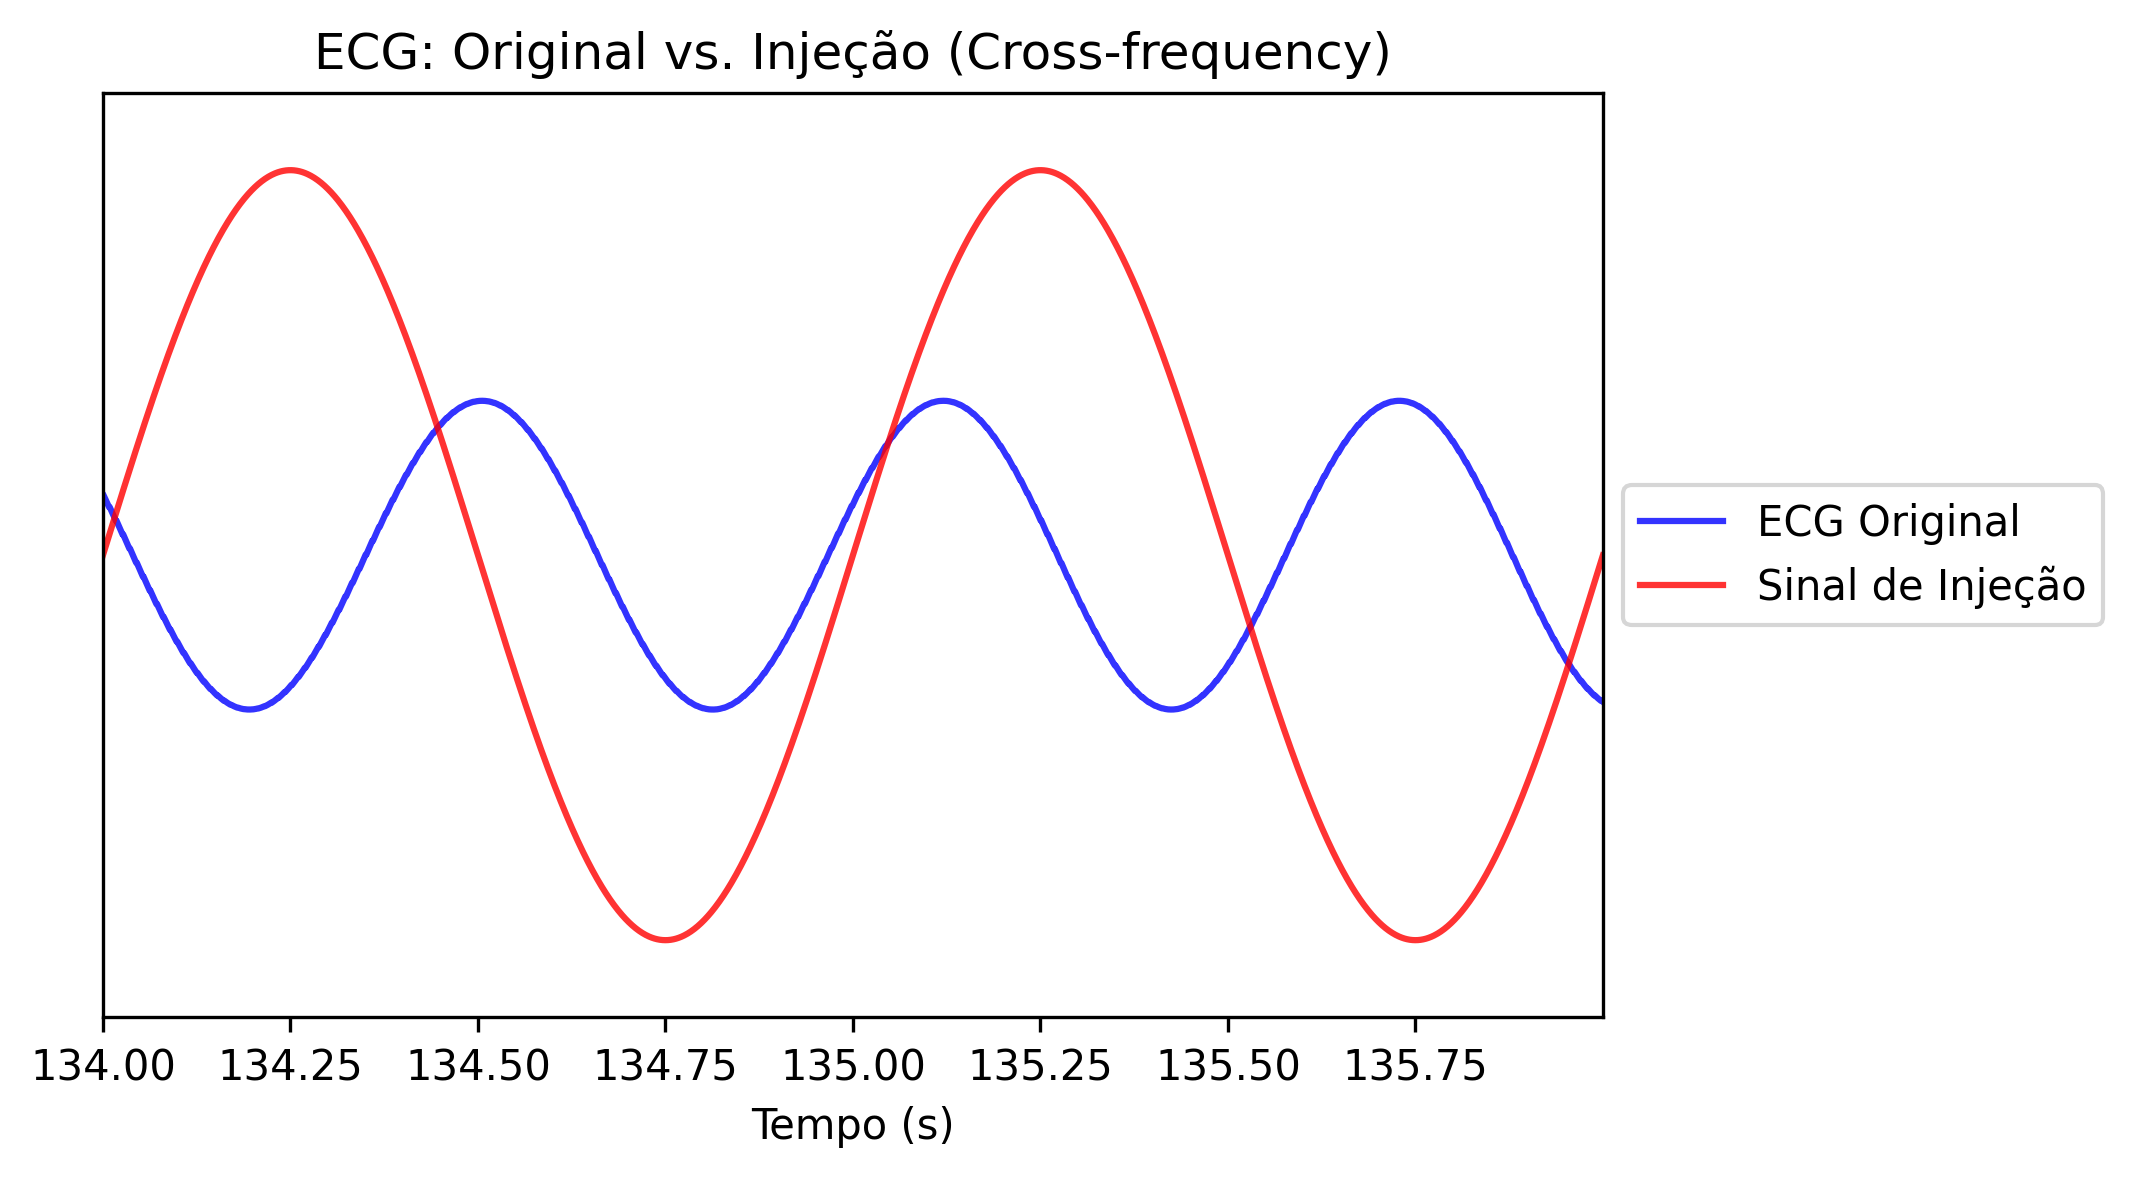
\includegraphics[width=0.8\textwidth]{figs/3_2_testing_connectivity_metrics/1_ECG_Original_vs_Injecao_Cross-frequency.png}
    \caption{ECG: comparação entre o sinal original e o sinal senoidal injetado (1~Hz), cenário Cross-frequency.}
    \label{fig:ecg_injection}
\end{figure}

\begin{figure}[htb]
    \centering
    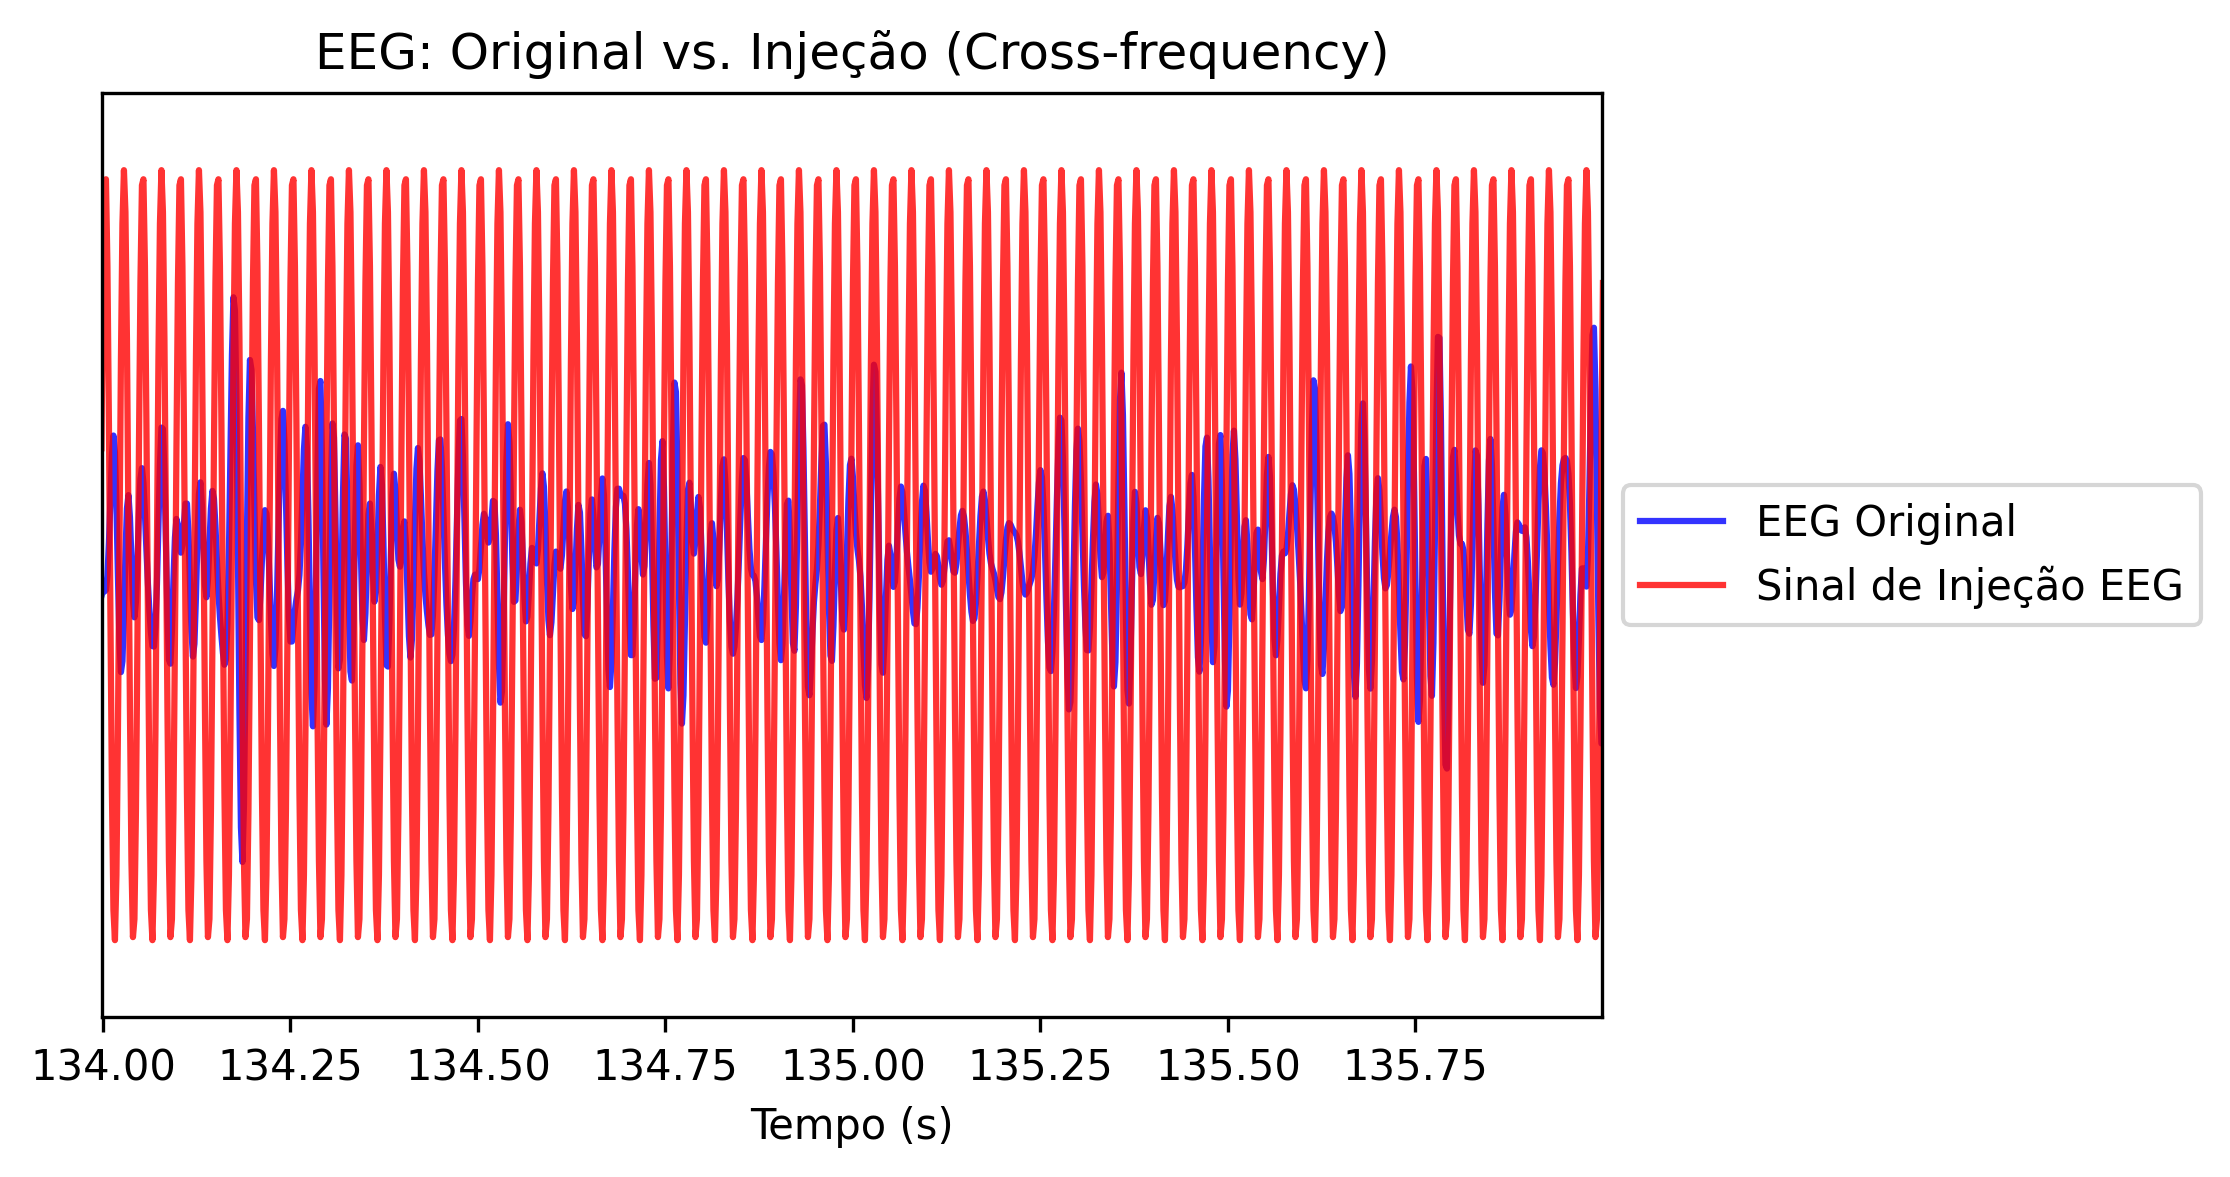
\includegraphics[width=0.8\textwidth]{figs/3_2_testing_connectivity_metrics/3_EEG_Original_vs_Injecao_Cross-frequency.png}
    \caption{EEG: comparação entre o sinal original e o sinal senoidal injetado (40~Hz), cenário Cross-frequency.}
    \label{fig:eeg_injection}
\end{figure}

No cenário Same-frequency, onde tanto o ECG quanto o EEG recebem sinais senoidais com a mesma frequência (10~Hz) mas com uma defasagem de \(\pi/4\), os resultados são ilustrados nas Figuras~\ref{fig:eeg_original_vs_injection_samefreq} e~\ref{fig:eeg_injected_samefreq}. Esses gráficos evidenciam a interferência gerada pela injeção controlada.

\begin{figure}[htb]
    \centering
    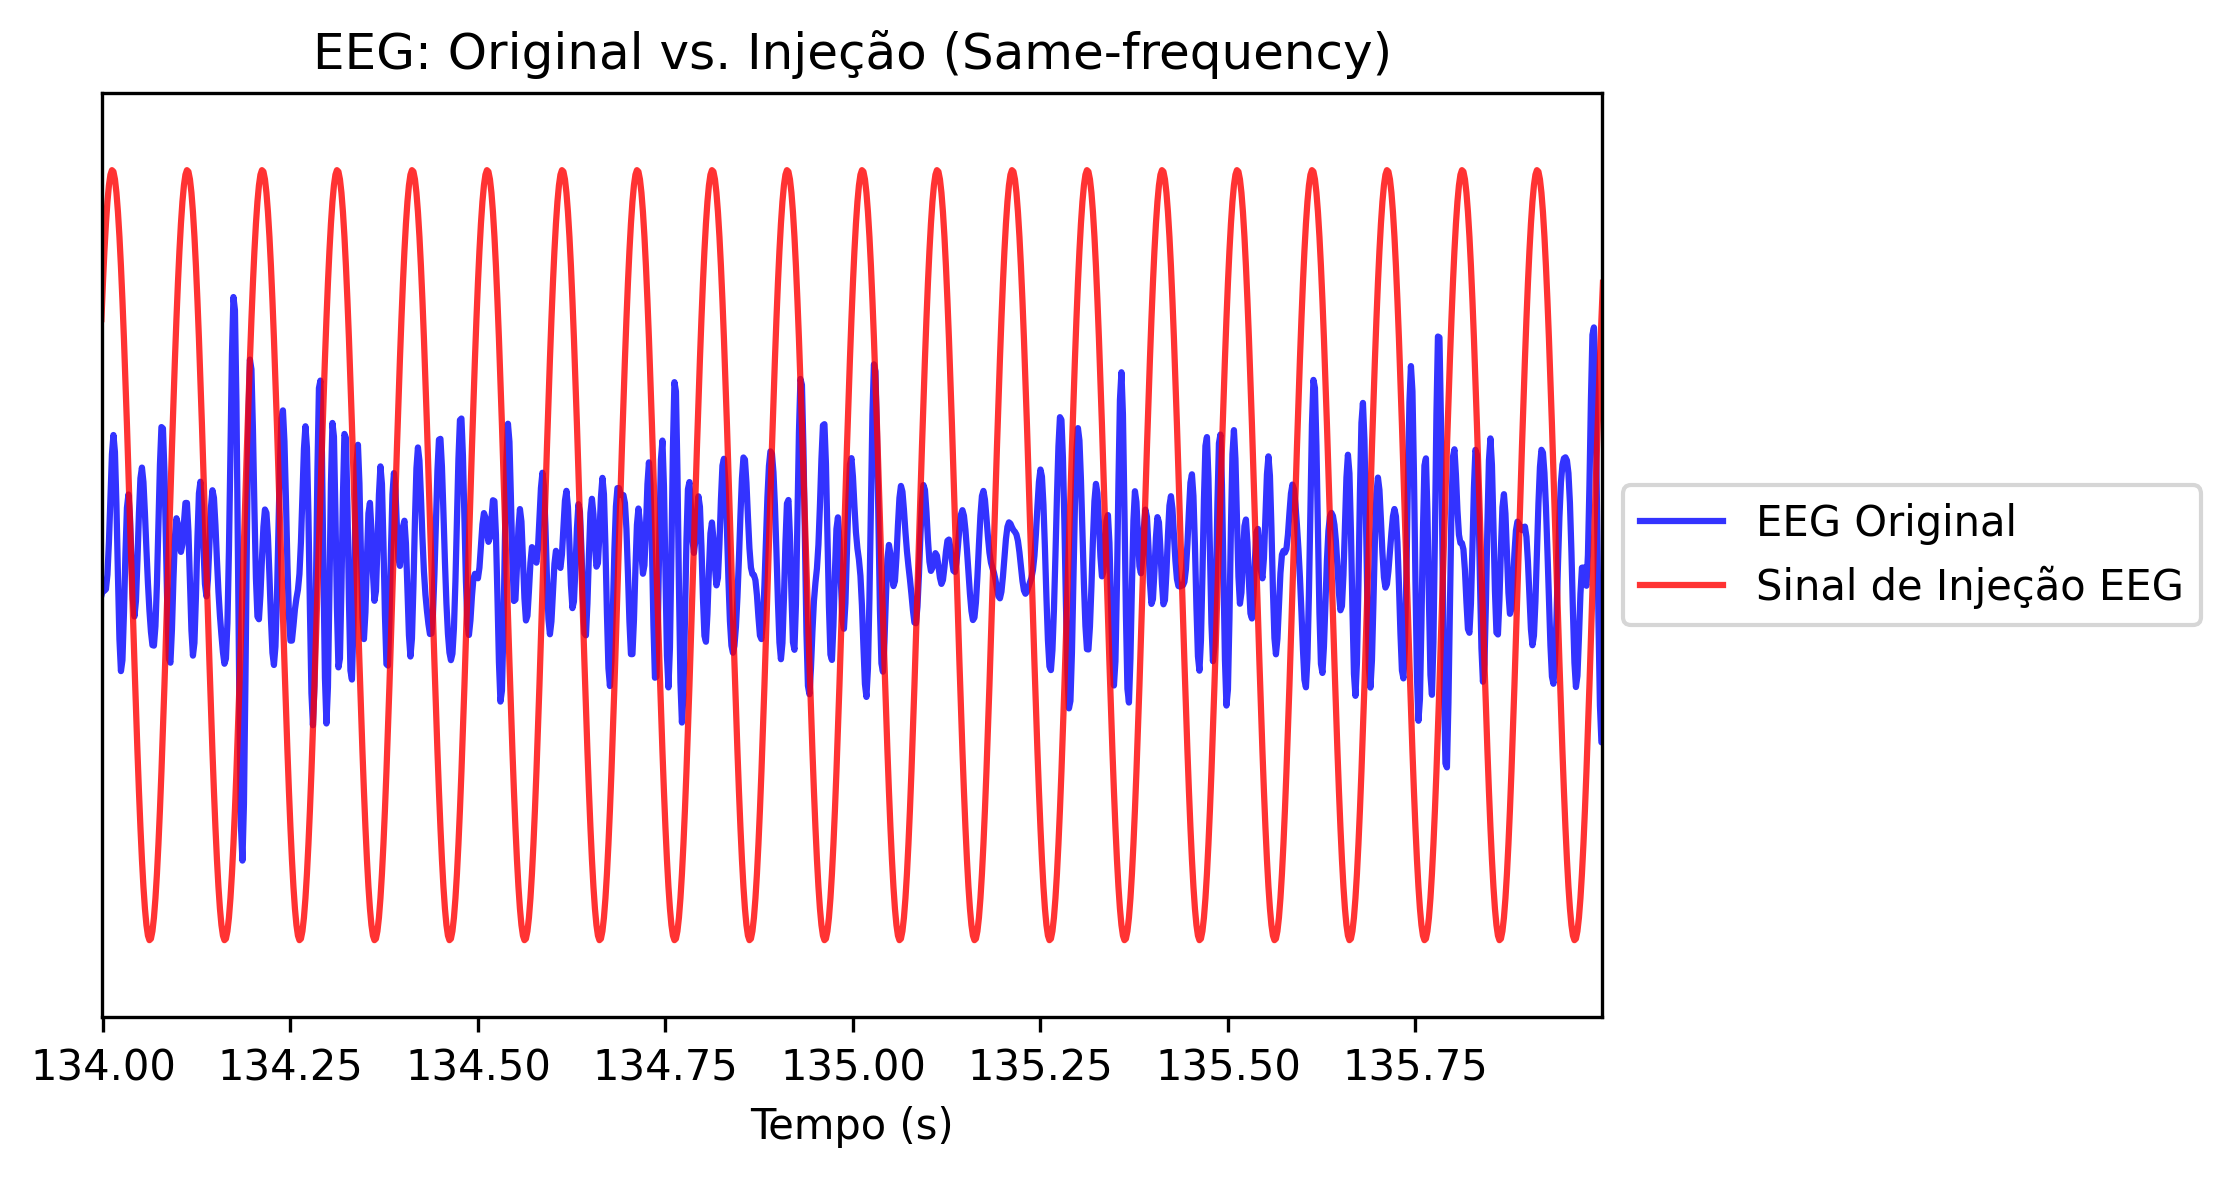
\includegraphics[width=0.8\textwidth]{figs/3_2_testing_connectivity_metrics/10_EEG_Original_vs_Injecao_Same-frequency.png}
    \caption{EEG original (azul) e sinal de injeção de 10 Hz (vermelho) com pequena defasagem (\(\pi/4\)).}
    \label{fig:eeg_original_vs_injection_samefreq}
\end{figure}

\begin{figure}[htb]
    \centering
    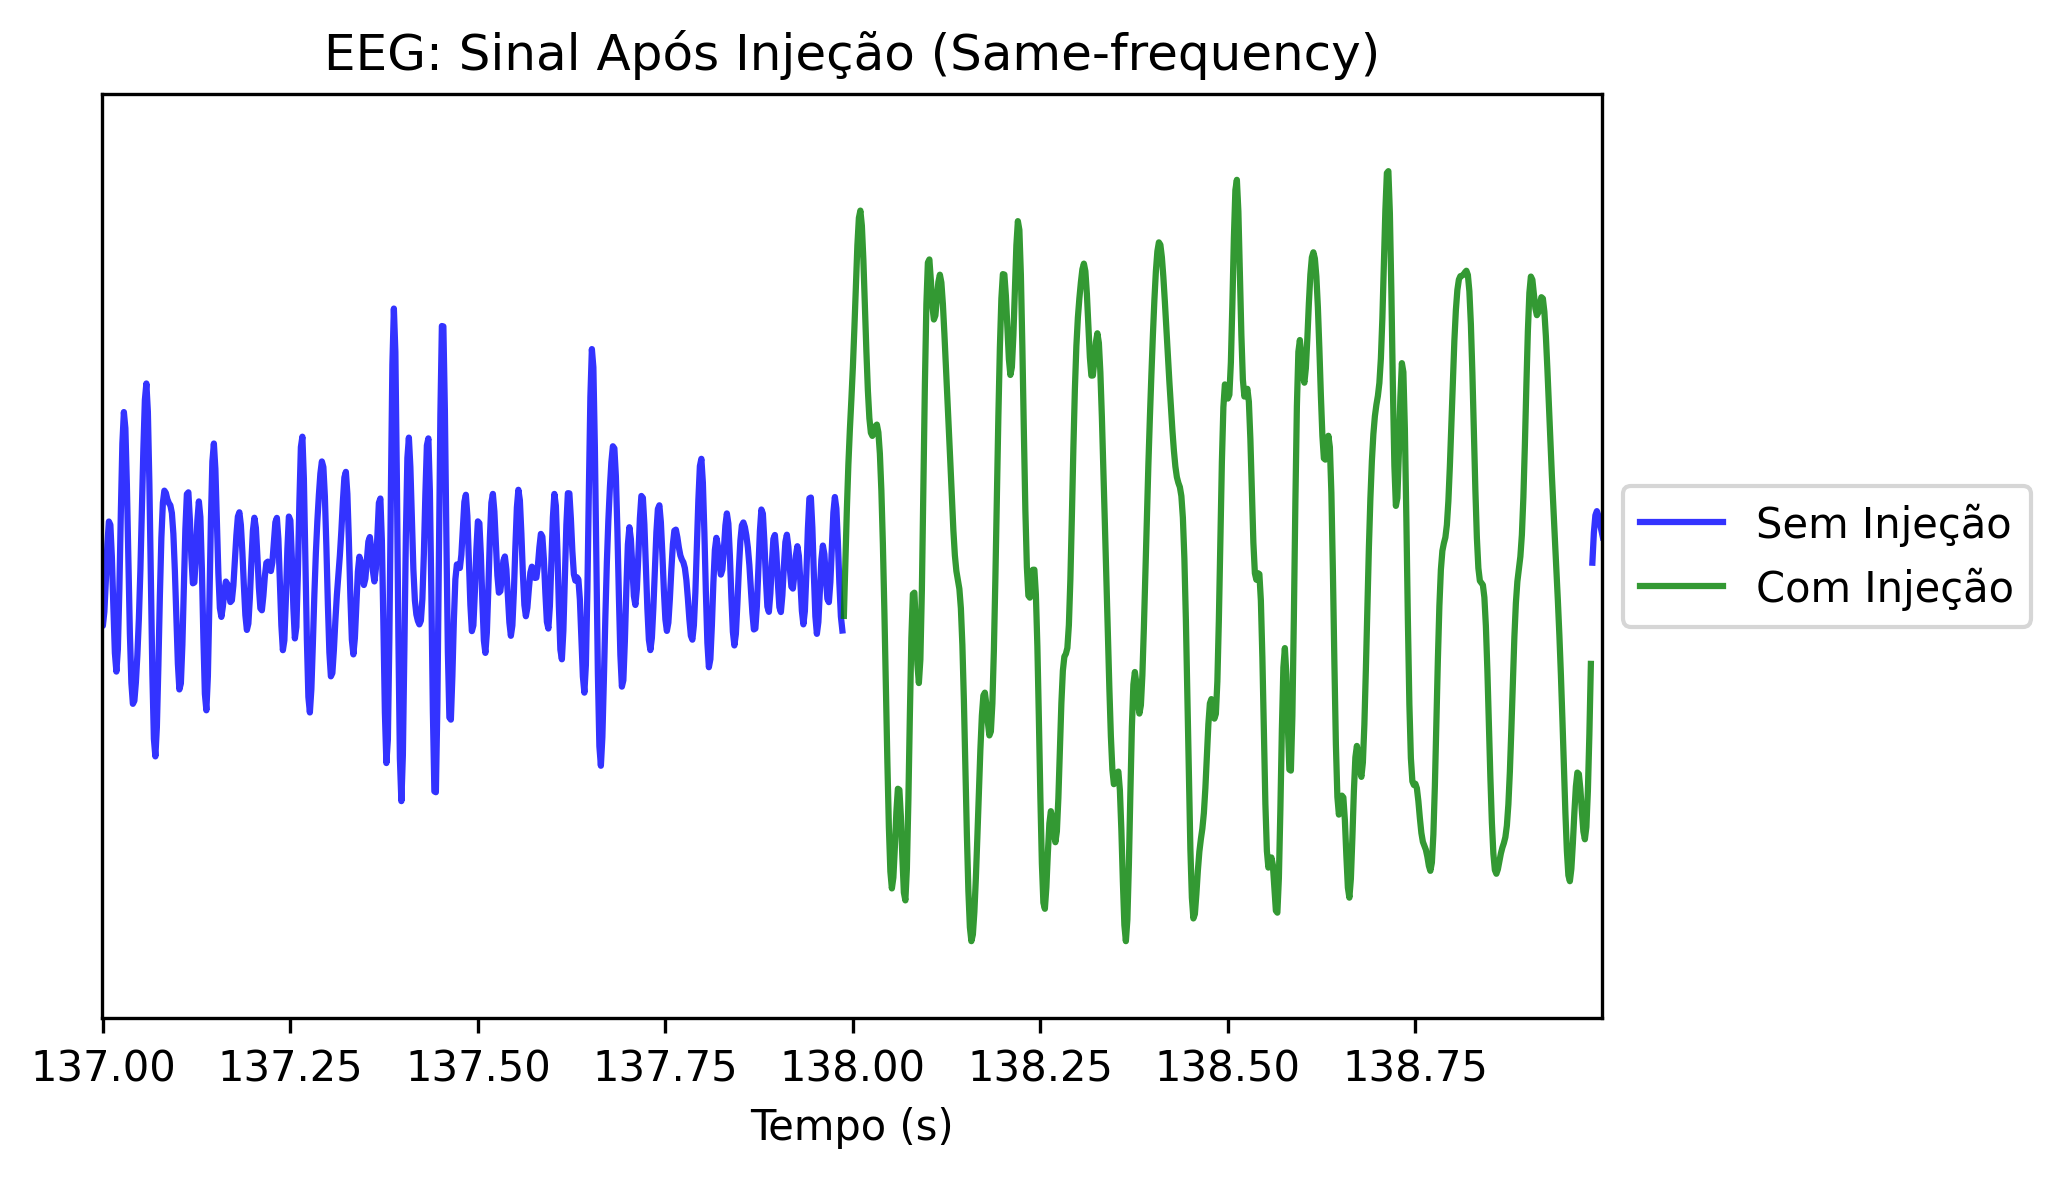
\includegraphics[width=0.8\textwidth]{figs/3_2_testing_connectivity_metrics/11_EEG_Injetado_Same-frequency.png}
    \caption{Sinal de EEG após a injeção controlada de uma senóide (verde), comparado ao sinal original sem injeção (azul).}
    \label{fig:eeg_injected_samefreq}
\end{figure}

Em seguida, extraímos as fases instantâneas utilizando a Transformada de Hilbert e geramos o sinal interferométrico, conforme exemplificado nas Figuras~\ref{fig:fases_instantaneas_samefreq} e~\ref{fig:sinal_interferometrico_samefreq}.

\begin{figure}[htb]
    \centering
    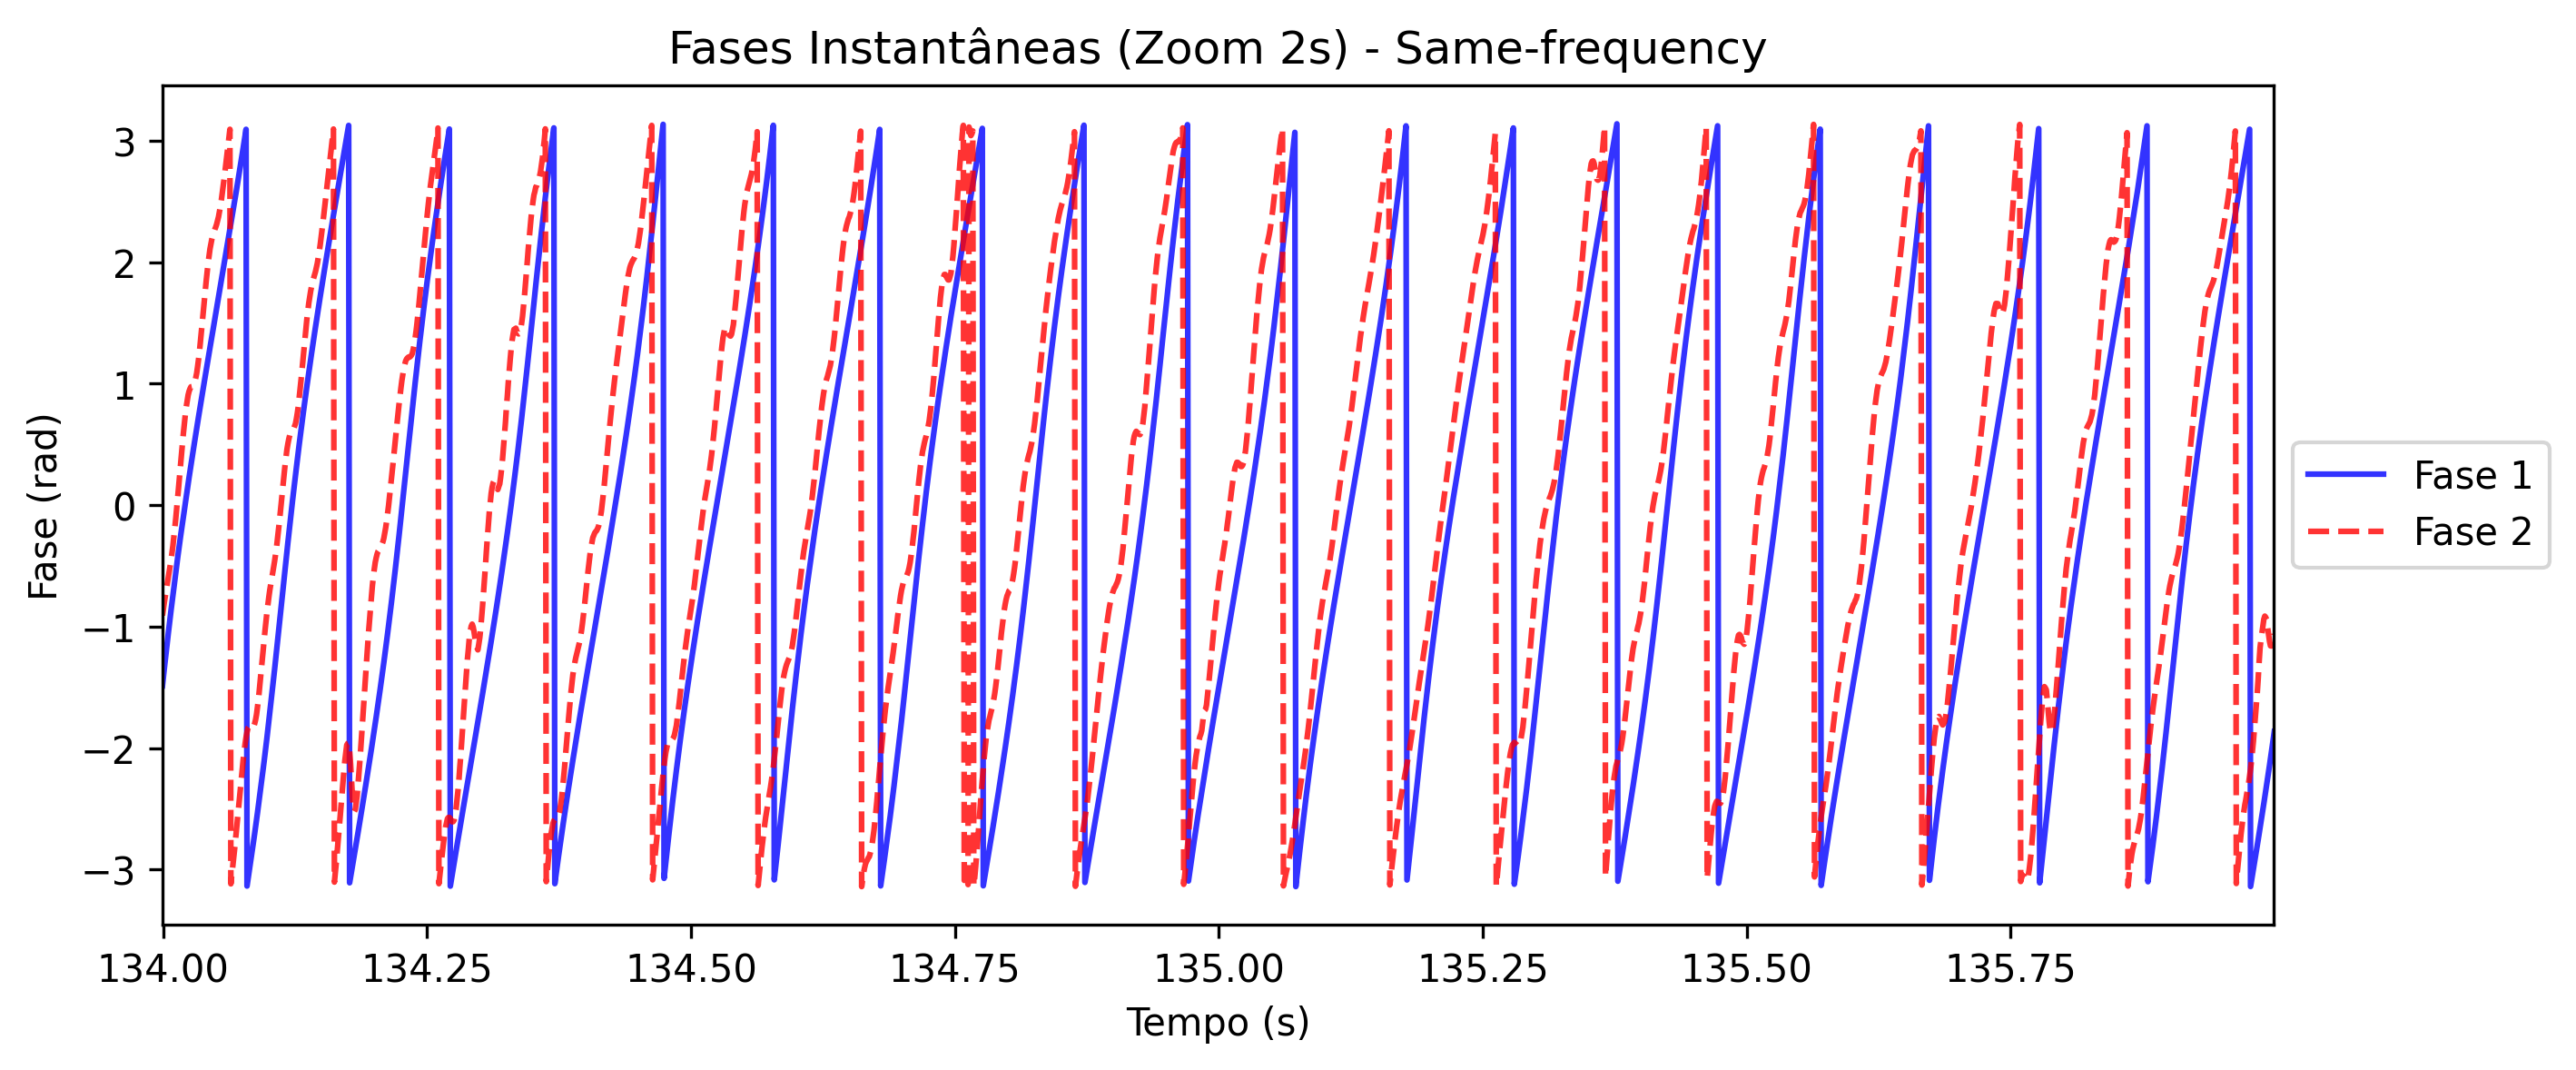
\includegraphics[width=0.8\textwidth]{figs/3_2_testing_connectivity_metrics/12_Passo1_Fases_Same-frequency.png}
    \caption{Fases instantâneas extraídas dos sinais EEG e ECG injetados (ambos a 10 Hz).}
    \label{fig:fases_instantaneas_samefreq}
\end{figure}

\begin{figure}[htb]
    \centering
    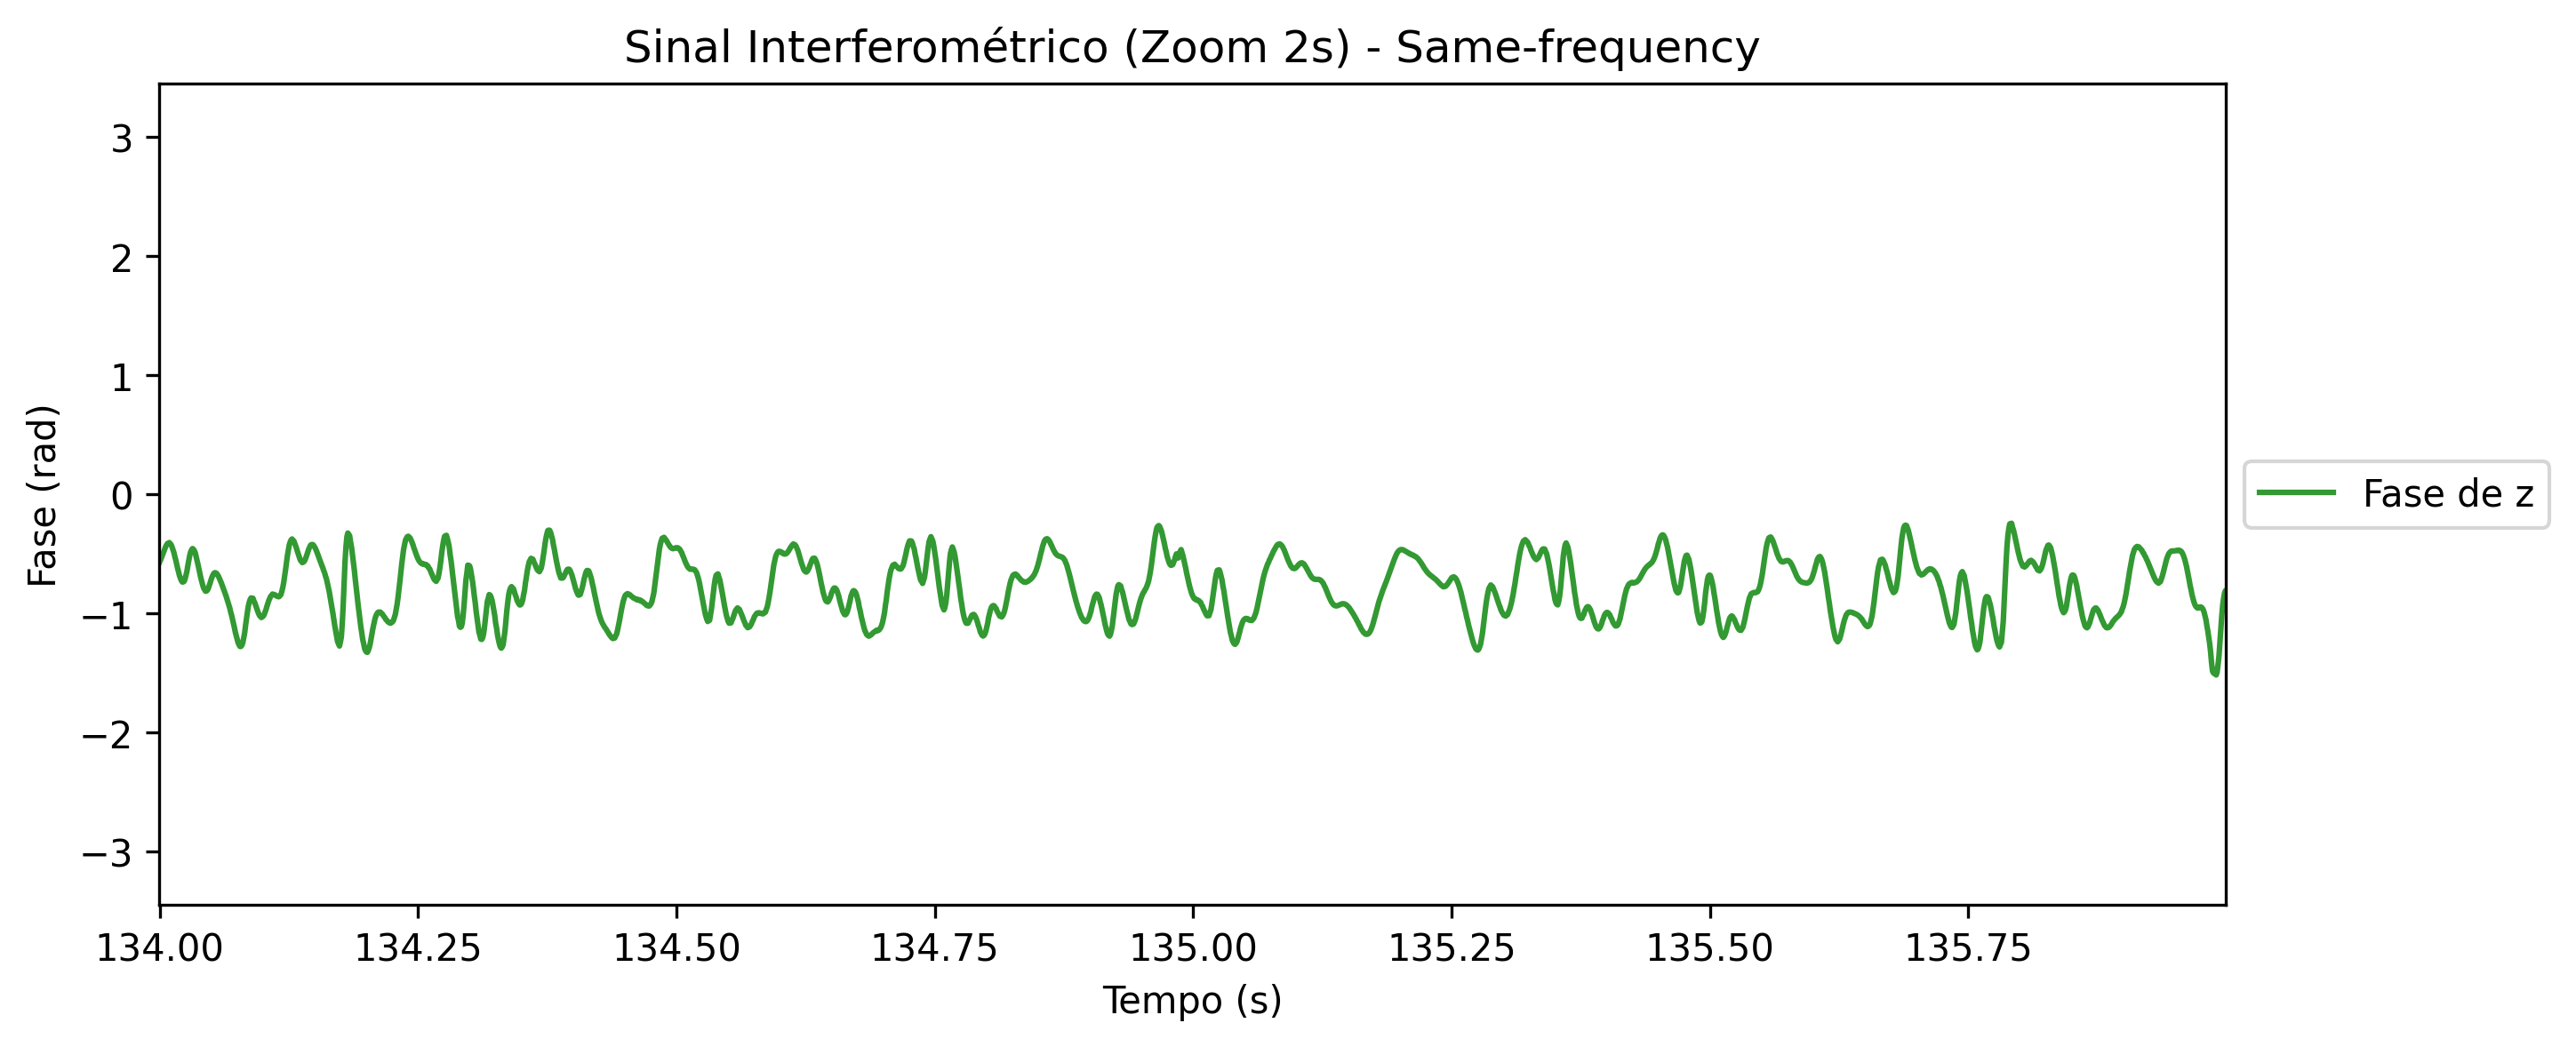
\includegraphics[width=0.8\textwidth]{figs/3_2_testing_connectivity_metrics/13_Passo2_Interferometrico_Same-frequency.png}
    \caption{Sinal interferométrico gerado pela diferença de fase instantânea (cenário Same-frequency).}
    \label{fig:sinal_interferometrico_samefreq}
\end{figure}

A seguir, calculamos o índice CF-PLM utilizando a Transformada de Fourier (FFT) sobre o sinal interferométrico. A Figura~\ref{fig:fft_psd_samefreq} exemplifica a análise, mostrando o pico em 0 Hz, que ocorre devido ao offset constante de fase entre os sinais de mesma frequência.

\begin{figure}[htb]
    \centering
    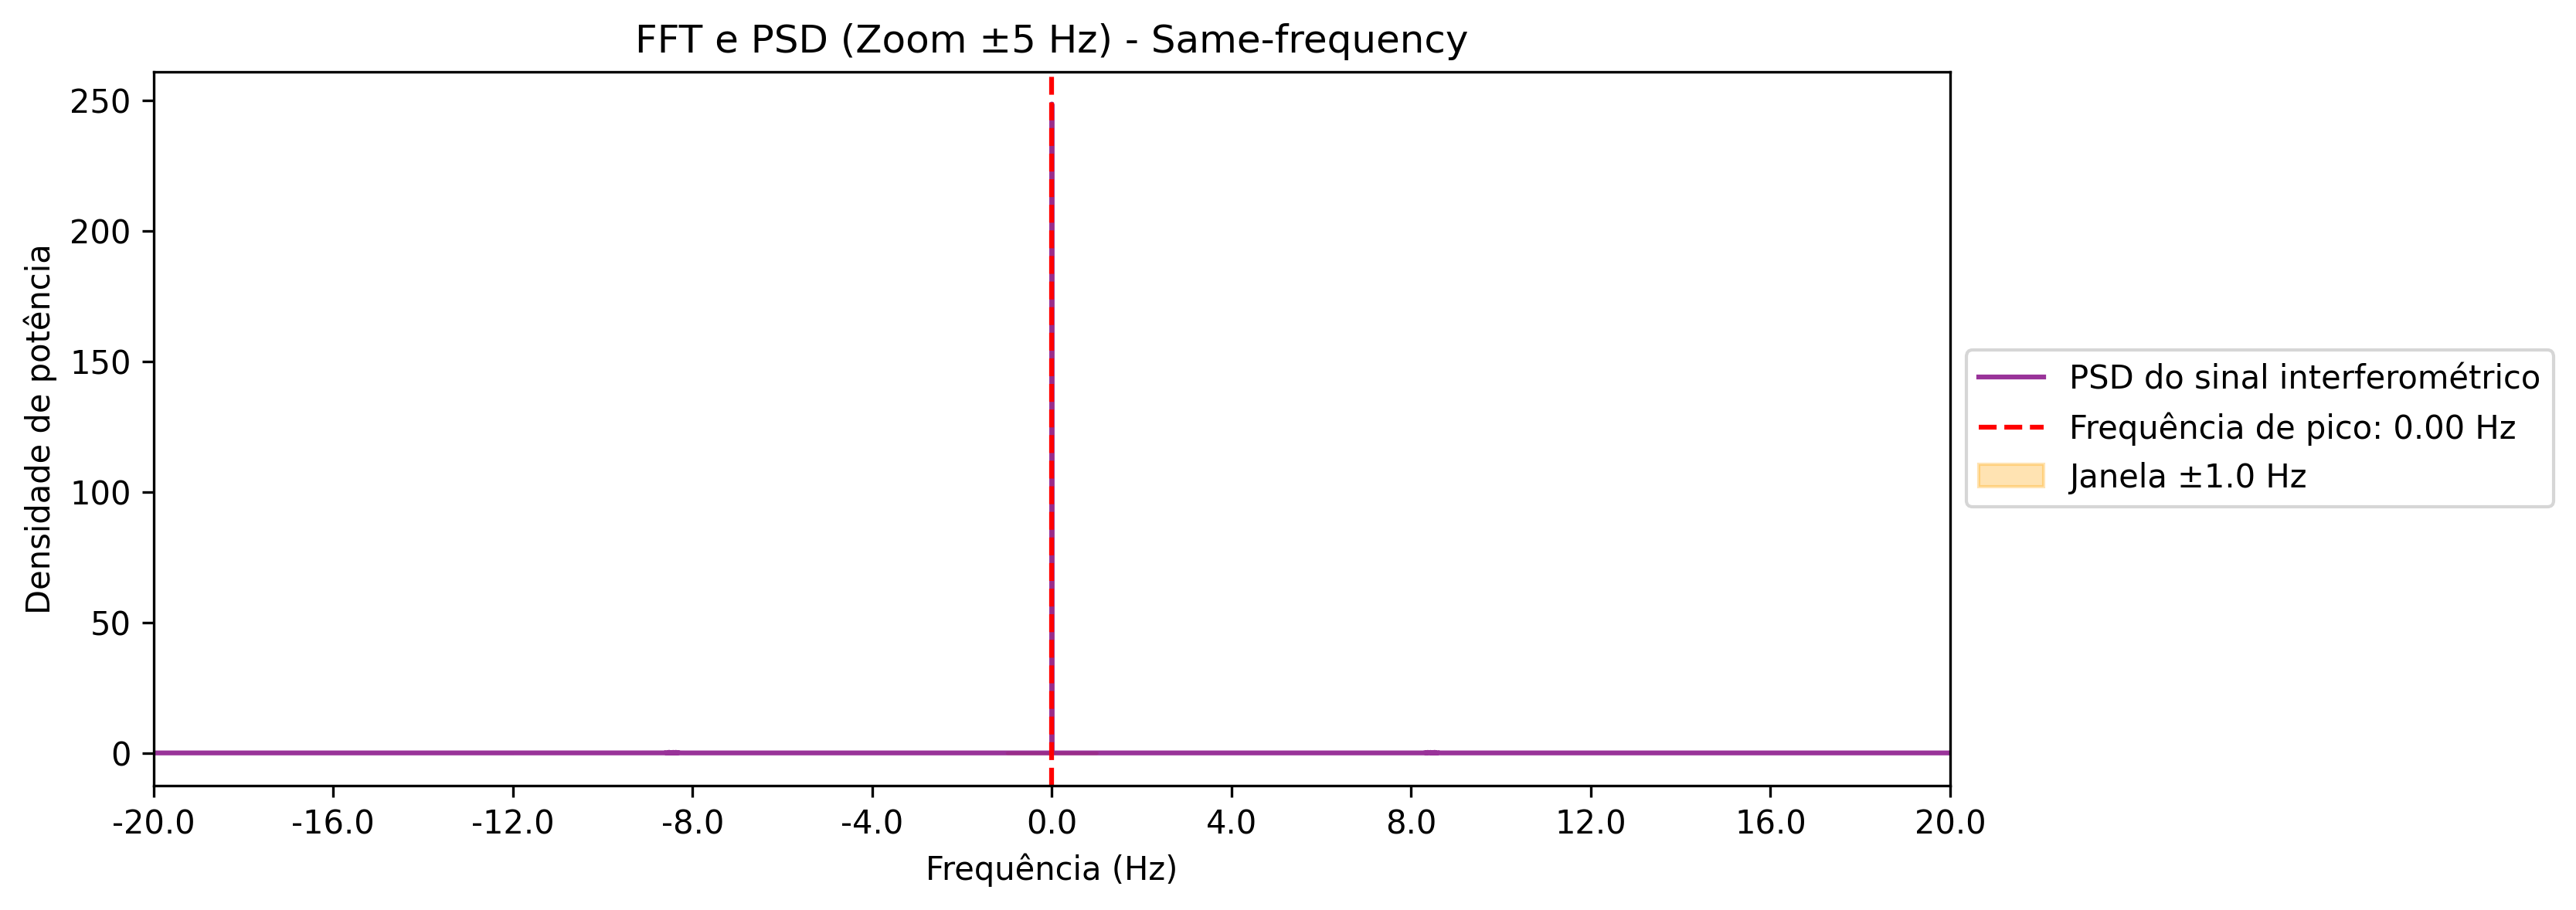
\includegraphics[width=0.8\textwidth]{figs/3_2_testing_connectivity_metrics/14_Passo3_FFT_PSD_Same-frequency.png}
    \caption{PSD do sinal interferométrico, indicando o pico em 0 Hz devido ao offset constante de fase entre os sinais de mesma frequência.}
    \label{fig:fft_psd_samefreq}
\end{figure}

Por fim, analisamos o cenário especial "Same-frequency com Phase Lag Zero", onde as fases dos sinais estão perfeitamente sincronizadas. As Figuras~\ref{fig:zerolag_phases_final} e~\ref{fig:zerolag_difference_final} demonstram que, nesse caso, a diferença de fase se aproxima de zero, evidenciando a robustez do PLI contra sincronizações triviais.

\begin{figure}[htb]
    \centering
    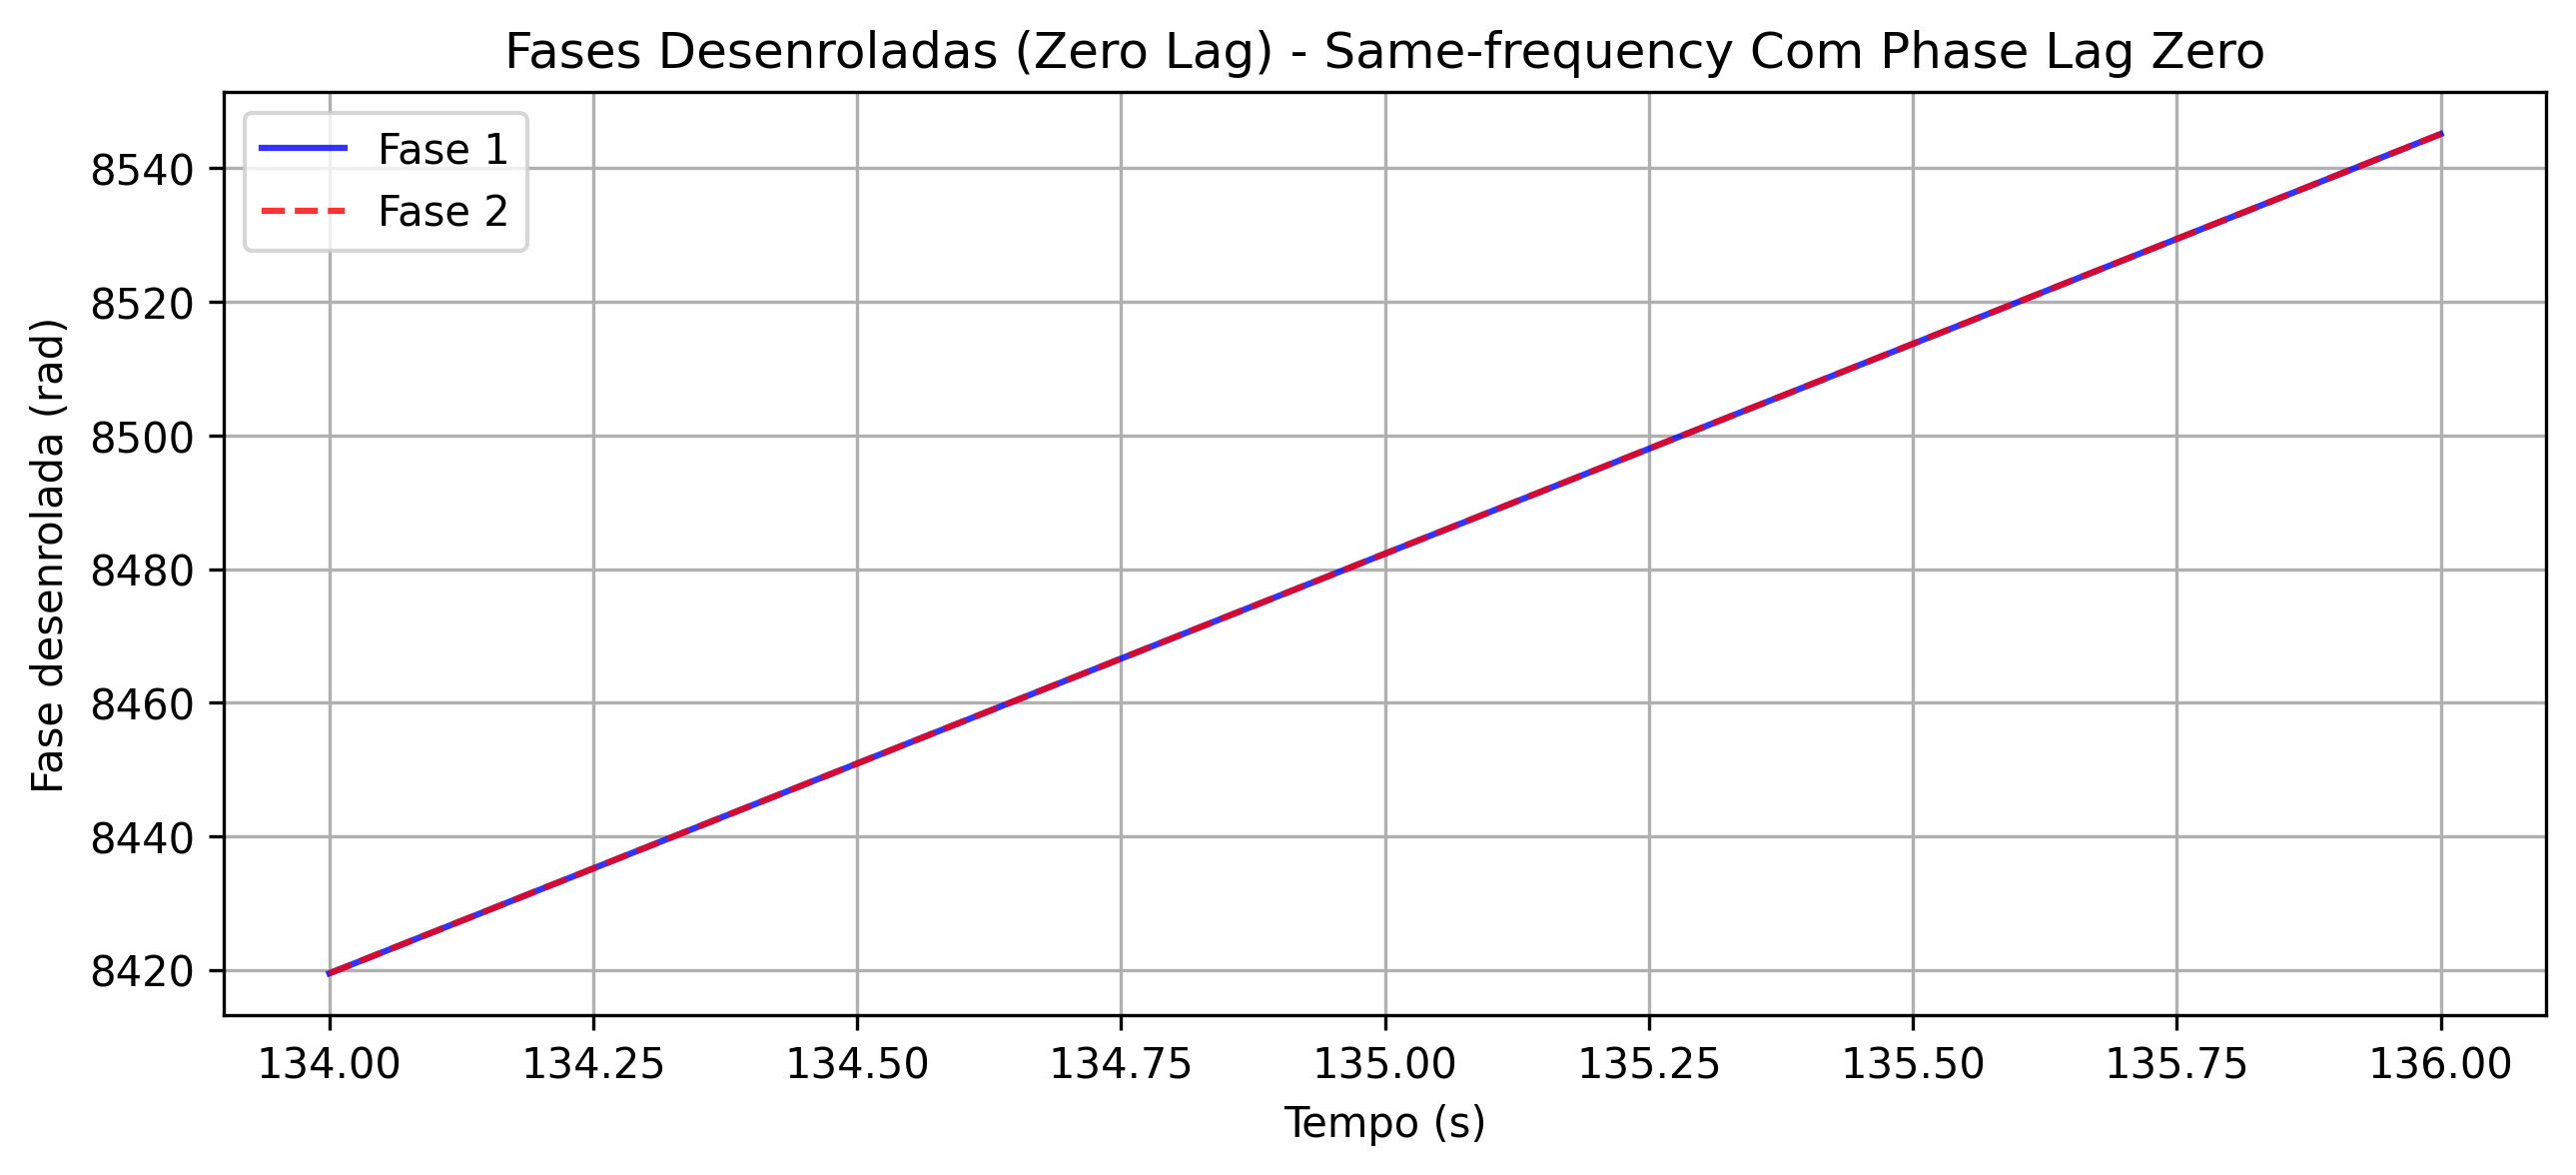
\includegraphics[width=0.8\textwidth]{figs/3_2_testing_connectivity_metrics/15_ZeroLag_Fases_Same-frequency Com Phase Lag Zero.png}
    \caption{Fases desenroladas em cenário sem defasagem (10 Hz), com sobreposição quase exata dos sinais.}
    \label{fig:zerolag_phases_final}
\end{figure}

\begin{figure}[htb]
    \centering
    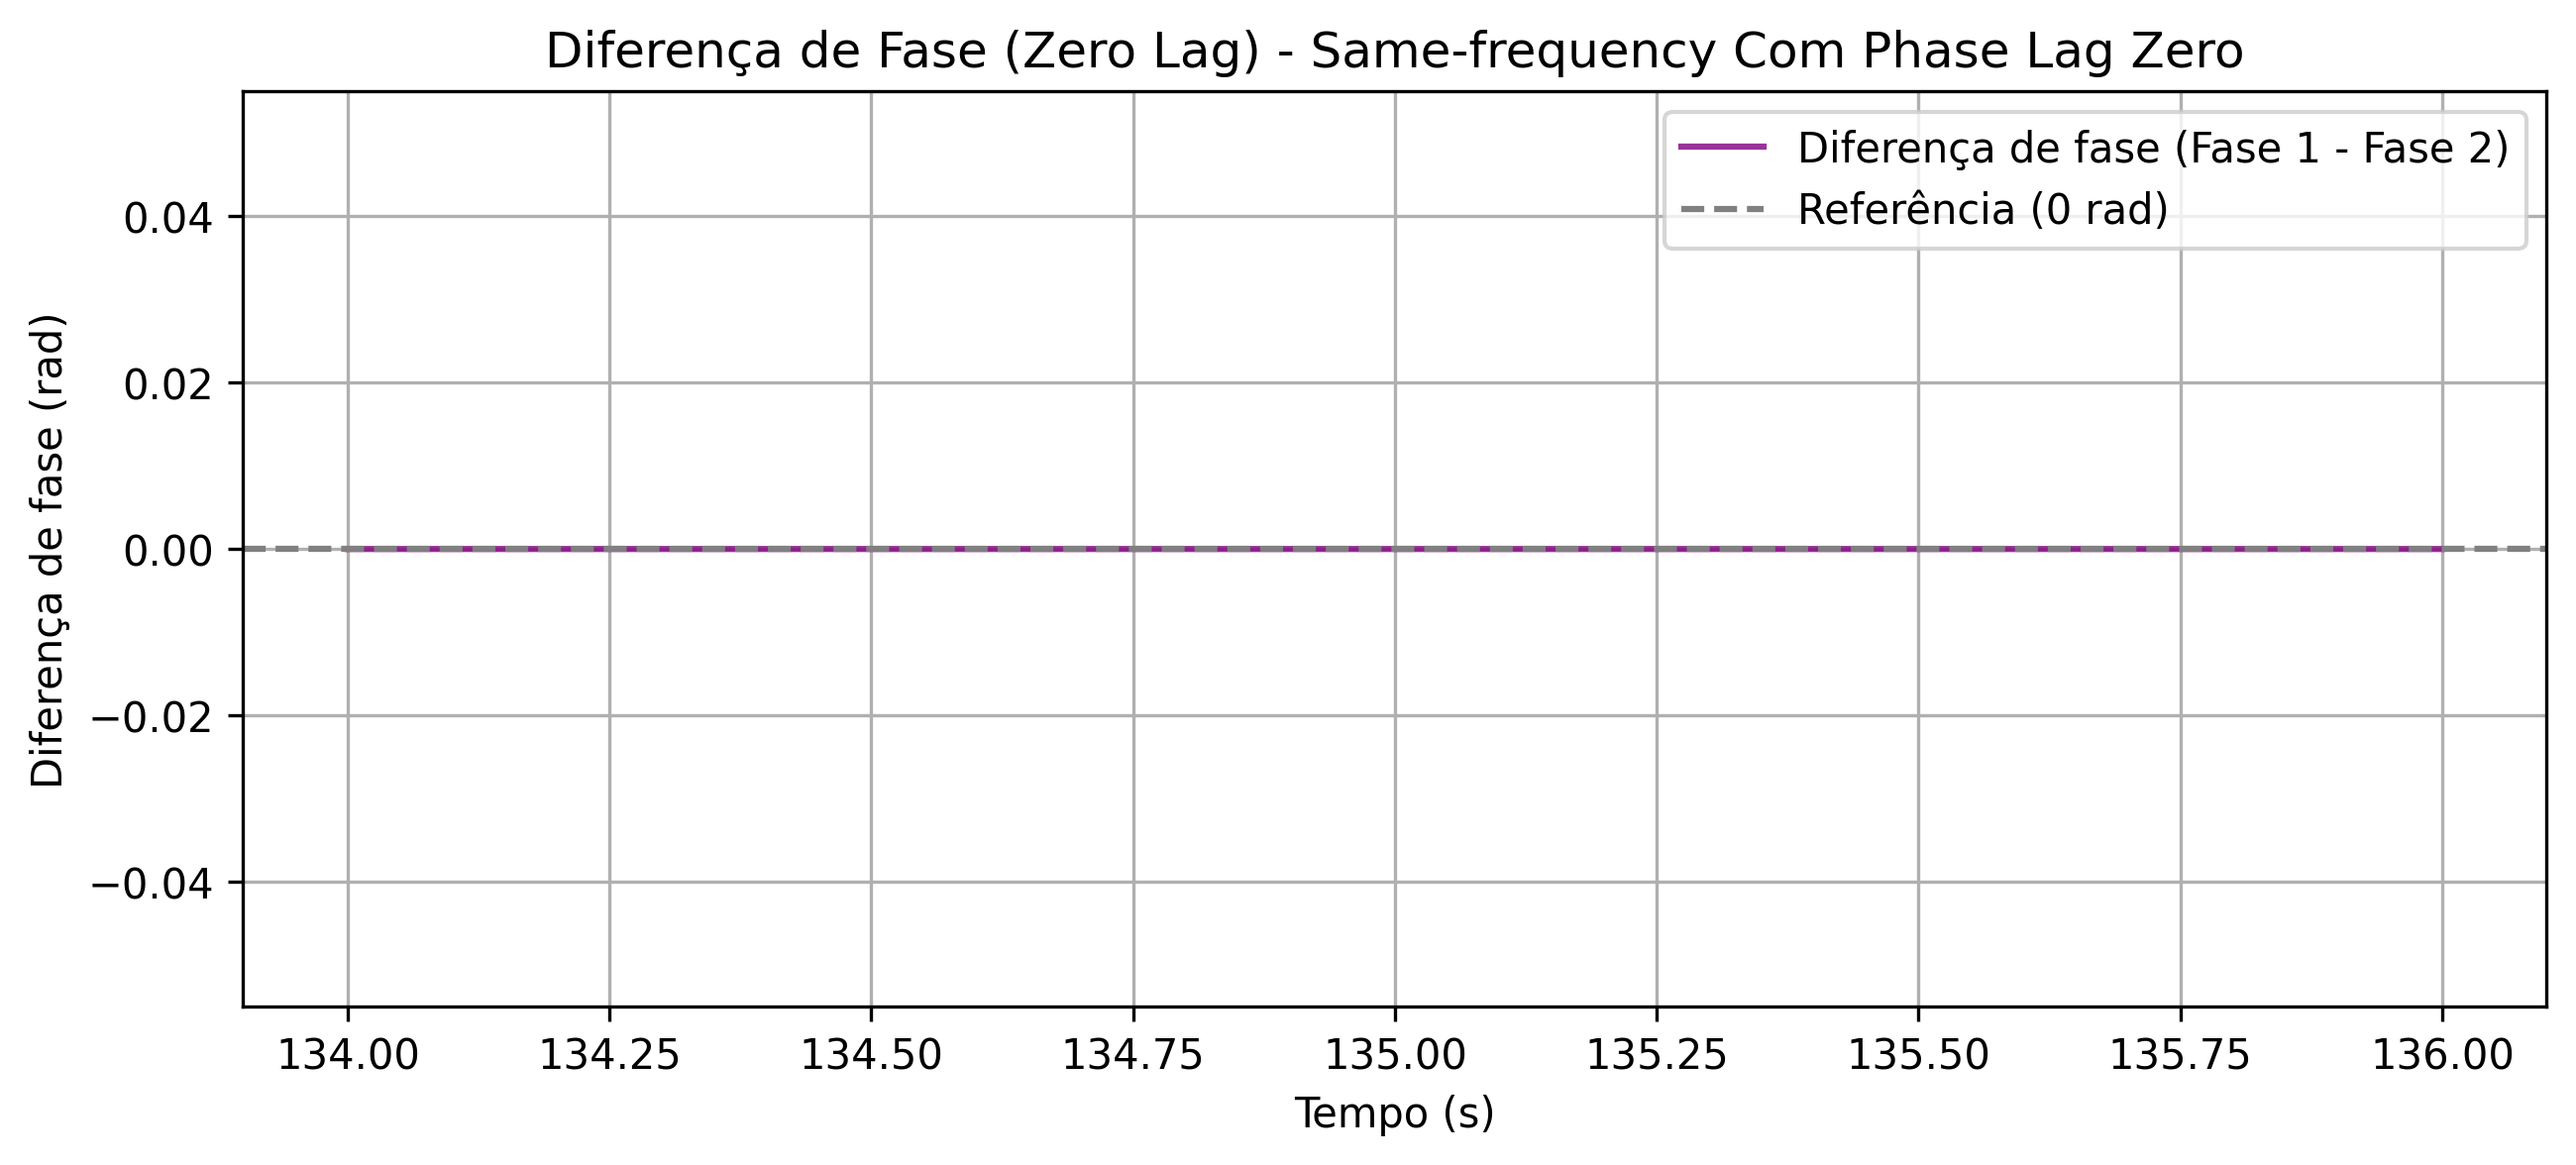
\includegraphics[width=0.8\textwidth]{figs/3_2_testing_connectivity_metrics/16_ZeroLag_Diferenca_Fase_Same-frequency Com Phase Lag Zero.png}
    \caption{Diferença de fase próxima a zero, indicando ausência completa de defasagem no cenário de Phase Lag Zero.}
    \label{fig:zerolag_difference_final}
\end{figure}

O comportamento geral dos índices CF-PLM, PLV e PLI nos diferentes cenários e níveis de injeção é resumido na Figura~\ref{fig:comparativo_metricas}.

\begin{figure}[htb]
    \centering
    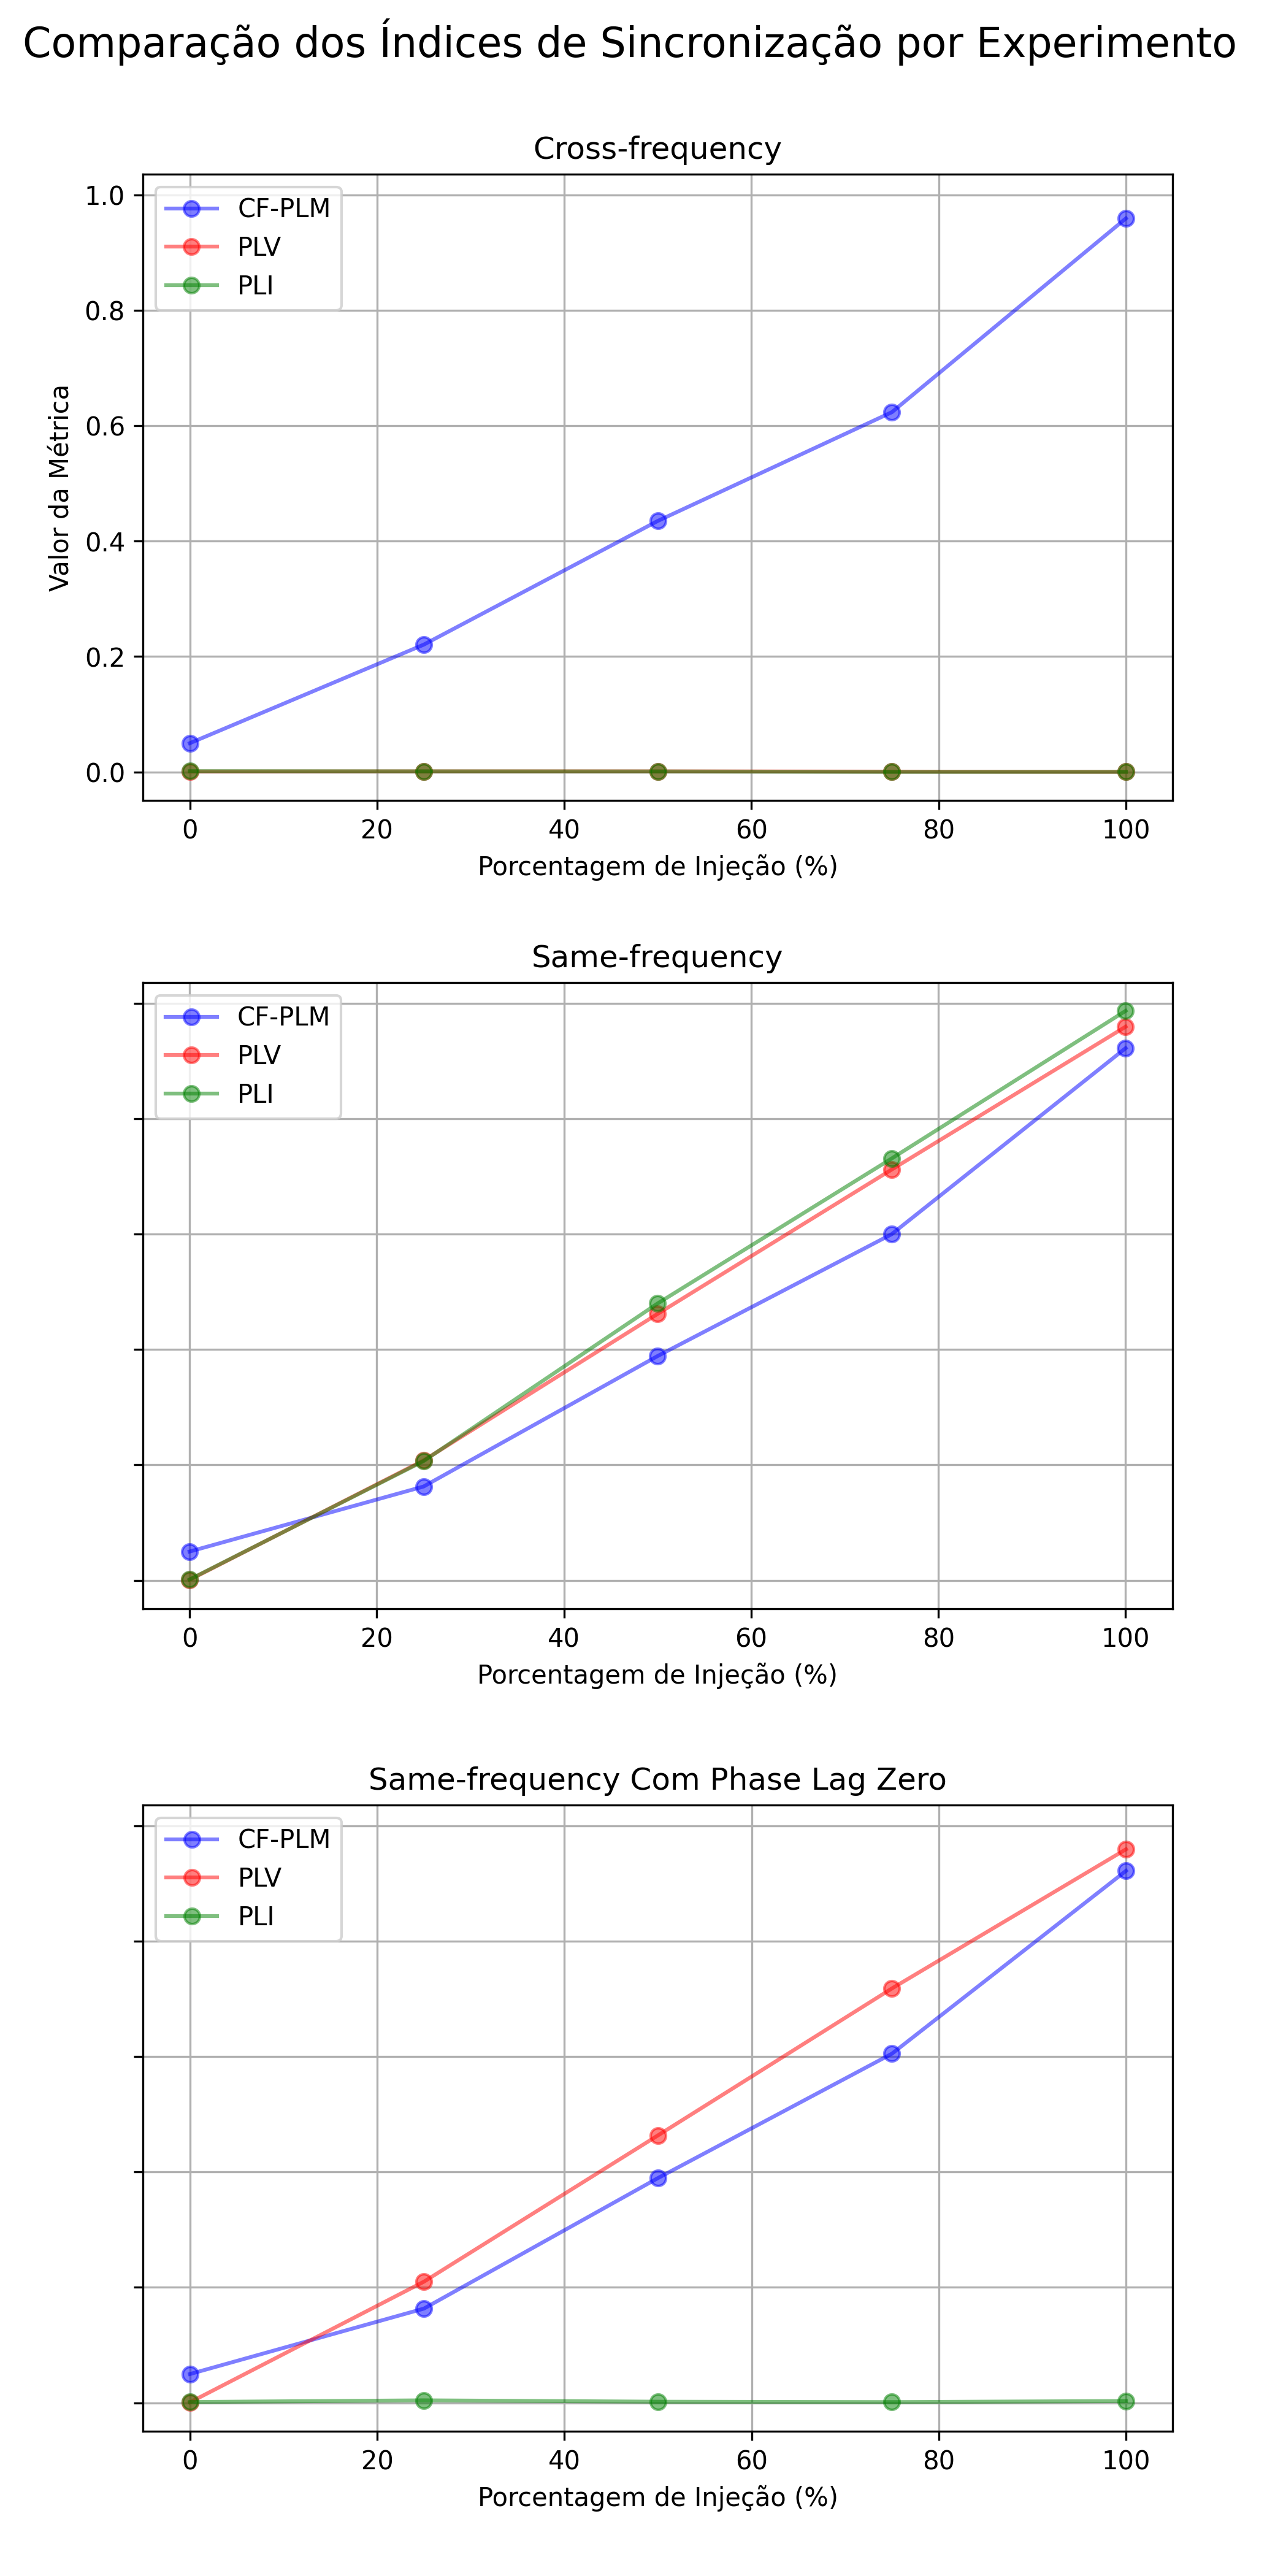
\includegraphics[width=\textwidth]{figs/3_2_testing_connectivity_metrics/17_Comparativo_Subplots_Experimentos.png}
    \caption{Comparação dos índices CF-PLM, PLV e PLI nos três cenários estudados, em função da porcentagem de injeção aplicada.}
    \label{fig:comparativo_metricas}
\end{figure}

Esses resultados justificam a escolha do CF-PLM para a análise de sincronização entre EEG e ECG (cross-frequency) e do PLI para sincronização em frequências iguais, evitando a detecção de acoplamentos triviais, como os decorrentes de volume conduction (phase lag zero). O PLV é reportado apenas para referência complementar, dada sua elevada sensibilidade em condições triviais.

\section{Análise de Conectividade ao Longo do Tempo}
\label{sec:connectivity_over_time}

Para investigar a dinâmica da sincronização ao longo da sessão experimental, os sinais foram segmentados em janelas de 10 segundos, considerando a gravação total de 4 minutos e 30 segundos de cada coleta. Em cada janela, foi calculada uma medida de sincronicidade (PLI, PLV ou CF-PLM) para cada par de canais, para cada banda de frequência, para cada condição (cathodic e sham) e para cada atleta. Em seguida, extraiu-se a mediana desses valores, fornecendo uma medida robusta da conectividade ao longo do tempo para cada configuração. Estudos recentes, como o de \citet{didaci2024how}, demonstraram que o tamanho da janela influencia significativamente a performance das métricas de conectividade em sistemas biométricos baseados em EEG, indicando que janelas entre 8 e 12 segundos oferecem um equilíbrio ideal entre precisão e estabilidade dos dados. Essa evidência reforça a estratégia adotada neste estudo.

Essa abordagem permite visualizar a evolução temporal da sincronização e comparar a estabilidade dos diferentes índices. Ressalta-se que, em nossas análises, enfatizamos o \emph{Wilcoxon RBC} e o p-valor corrigido por Bonferroni como principais indicadores de tamanho de efeito e significância estatística, respectivamente, dada sua robustez em contextos não paramétricos e na presença de variabilidade e outliers.

A seguir, apresentamos as séries temporais obtidas para três métricas principais:

\begin{itemize}
    \item \textbf{CF-PLM (EEG-ECG):} A Figura~\ref{fig:cfplm_time_cat} mostra a mediana do CF-PLM ao longo do tempo para a condição cathodic, refletindo a sincronização cross-frequency entre EEG e ECG.
    \item \textbf{PLI (EEG-EEG):} A Figura~\ref{fig:pli_time_cat} apresenta a mediana do PLI ao longo do tempo para a condição cathodic, indicando a sincronização iso-frequencial entre canais cerebrais.
    \item \textbf{PLV (EEG-EEG):} A Figura~\ref{fig:plv_time_cat} exibe a mediana do PLV ao longo do tempo para a condição cathodic, utilizada aqui para comparação, considerando que o PLV é mais sensível a ruídos e aos efeitos de volume conduction.
\end{itemize}

Cada gráfico é construído a partir dos valores calculados em janelas de 10 segundos, onde a mediana de cada janela representa a medida de sincronicidade de forma robusta, minimizando o impacto de variações pontuais e outliers.

\begin{figure}[htb]
    \centering
    \includegraphics[width=0.8\textwidth]{figs/4_connectivity_over_time/Mediana_do_CF-PLM_ao_longo_do_tempo_(EEG_ECG)_Catódica.png}
    \caption{Mediana do CF-PLM ao longo do tempo para a condição cathodic (EEG-ECG). Cada ponto representa a mediana da medida de sincronicidade calculada em janelas de 10 segundos, evidenciando a evolução do acoplamento cross-frequency entre EEG e ECG.}
    \label{fig:cfplm_time_cat}
\end{figure}

\begin{figure}[htb]
    \centering
    \includegraphics[width=0.8\textwidth]{figs/4_connectivity_over_time/Mediana_do_PLI_ao_longo_do_tempo_(EEG_EEG)_Catódica.png}
    \caption{Mediana do PLI ao longo do tempo para a condição cathodic (EEG-EEG). O gráfico mostra como a sincronização iso-frequencial entre canais cerebrais varia ao longo da gravação.}
    \label{fig:pli_time_cat}
\end{figure}

\begin{figure}[htb]
    \centering
    \includegraphics[width=0.8\textwidth]{figs/4_connectivity_over_time/Mediana_do_PLV_ao_longo_do_tempo_(EEG_EEG)_Catódica.png}
    \caption{Mediana do PLV ao longo do tempo para a condição cathodic (EEG-EEG). Este índice é apresentado para comparação com o PLI, embora seja mais sensível a ruídos e efeitos de volume conduction.}
    \label{fig:plv_time_cat}
\end{figure}